\documentclass[mat2, tisk]{fmfdelo}
% \documentclass[fin2, tisk]{fmfdelo}
% \documentclass[isrm2, tisk]{fmfdelo}
% \documentclass[ped, tisk]{fmfdelo}
% Če pobrišete možnost tisk, bodo povezave obarvane,
% na začetku pa ne bo praznih strani po naslovu, …

%%%%%%%%%%%%%%%%%%%%%%%%%%%%%%%%%%%%%%%%%%%%%%%%%%%%%%%%%%%%%%%%%%%%%%%%%%%%%%%
% METAPODATKI
%%%%%%%%%%%%%%%%%%%%%%%%%%%%%%%%%%%%%%%%%%%%%%%%%%%%%%%%%%%%%%%%%%%%%%%%%%%%%%%

% - vaše ime
\avtor{Uroš Kosmač}

% - naslov dela v slovenščini
\naslov{Turbulence v atmosferi in Large eddy simulacije}

% - naslov dela v angleščini
\title{Atmospheric turbulence and Large eddy simulations}

% - ime mentorja/mentorice s polnim nazivom:
%   - doc.~dr.~Ime Priimek
%   - izr.~prof.~dr.~Ime Priimek
%   - prof.~dr.~Ime Priimek
%   za druge variante uporabite ustrezne ukaze
\mentor{prof.~dr.~Emil Žagar}
\somentor{dr.~Peter Smerkol}
% \mentorica{...}
% \somentorica{...}
% \mentorja{...}{...}
% \somentorja{...}{...}
% \mentorici{...}{...}
% \somentorici{...}{...}

% - leto magisterija
\letnica{2024}

% - povzetek v slovenščini
%   V povzetku na kratko opišite vsebinske rezultate dela. Sem ne sodi razlaga
%   organizacije dela, torej v katerem razdelku je kaj, pač pa le opis vsebine.
\povzetek{Tukaj napišemo povzetek vsebine. Sem sodi razlaga vsebine in ne opis tega, kako je delo organizirano.}

% - povzetek v angleščini
\abstract{An abstract of the work is written here. This includes a short description of
the content and not the structure of your work.}

% - klasifikacijske oznake, ločene z vejicami
%   Oznake, ki opisujejo področje dela, so dostopne na strani https://www.ams.org/msc/
\klasifikacija{74B05, 65N99}

% - ključne besede, ki nastopajo v delu, ločene s \sep
\kljucnebesede{integracija\sep kompleks\sep \texorpdfstring{$C^*$}{C*}-algebre}

% - angleški prevod ključnih besed
\keywords{integration\sep complex\sep \texorpdfstring{$C^*$}{C*}-algebras}

% - neobvezna zahvala
%\zahvala{
%  Neobvezno.
%  Zahvaljujem se \dots
%}

% - program dela, ki ga napiše mentor z osnovno literaturo
\programdela{
  Mentor naj napiše program dela skupaj z osnovno literaturo.
}

\osnovnaliteratura{
% Literatura mora biti tukaj posebej samostojno navedena (po pomembnosti) in ne
% le citirana. V tem razdelku literature ne oštevilčimo po svoje, ampak uporabljamo
% ukaz \vnosliterature, v katerega vpišemo citat
  \vnosliterature{wyngaard}
  %\vnosliterature{lebedev2009introduction}
  %\vnosliterature{gurtin1982introduction}
  %\vnosliterature{zienkiewicz2000finite}
  %\vnosliterature{STtemplate}
}

% - ime datoteke z viri (vključno s končnico .bib), če uporabljate BibTeX
\literatura{literatura.bib}

%%%%%%%%%%%%%%%%%%%%%%%%%%%%%%%%%%%%%%%%%%%%%%%%%%%%%%%%%%%%%%%%%%%%%%%%%%%%%%%
% DODATNE DEFINICIJE
%%%%%%%%%%%%%%%%%%%%%%%%%%%%%%%%%%%%%%%%%%%%%%%%%%%%%%%%%%%%%%%%%%%%%%%%%%%%%%%

% naložite dodatne pakete, ki jih potrebujete
\usepackage{units}        % fizikalne enote kot \unit[12]{kg} s polovico nedeljivega presledka, glej primer v kodi
\usepackage{graphicx}     % za slike
\usepackage{graphicx}
\usepackage{subcaption}
\usepackage{tikz}
\usepackage{tikz-3dplot}
\usepackage[utf8]{inputenc}
\usepackage[T1]{fontenc}
\usepackage{lmodern}
\usepackage{amsmath}
\usepackage{amsthm}
\usepackage{amsfonts}
\usepackage{amssymb}
\usepackage{enumitem}
\usepackage{commath}
\usepackage{mathtools}
\usepackage{adjustbox}
\usepackage{setspace}
\usepackage{bigints}
\usepackage{hyperref}
\usepackage{caption}
\usepackage{mathrsfs}
\usepackage[scr=boondoxo]{mathalpha}
\hypersetup{
  colorlinks=true,
  linkcolor=blue,
  urlcolor=cyan,
}
\usepackage{esdiff}
\usepackage{animate}
\usetikzlibrary{quotes,arrows.meta}
\usetikzlibrary{decorations.pathreplacing} 
\AtBeginDocument{\hypersetup{pdfborder={0 0 1.1}}}

% VEČ ZANIMIVIH PAKETOV
% \usepackage{array}      % več možnosti za tabele
% \usepackage[list=true,listformat=simple]{subcaption}  % več kot ena slika na figure, omogoči slika 1a, slika 1b
% \usepackage[all]{xy}    % diagrami
% \usepackage{doi}        % za clickable DOI entrye v bibliografiji
% \usepackage{enumerate}     % več možnosti za sezname

% Za barvanje source kode
% \usepackage{minted}
% \renewcommand\listingscaption{Program}

% Za pisanje psevdokode
% \usepackage{algpseudocode}  % za psevdokodo
% \usepackage{algorithm}
% \floatname{algorithm}{Algoritem}
% \renewcommand{\listalgorithmname}{Kazalo algoritmov}

% deklarirajte vse matematične operatorje, da jih bo LaTeX pravilno stavil
% \DeclareMathOperator{\...}{...}

% vstavite svoje definicije ...
\newcommand{\R}{\mathbb R}
\newcommand{\N}{\mathbb N}
\newcommand{\Z}{\mathbb Z}
% Lahko se zgodi, da je ukaz \C definiral že paket hyperref,
% zato dobite napako: Command \C already defined.
% V tem primeru namesto ukaza \newcommand uporabite \renewcommand
\newcommand{\C}{\mathbb C}
\newcommand{\Q}{\mathbb Q}

%%%%%%%%%%%%%%%%%%%%%%%%%%%%%%%%%%%%%%%%%%%%%%%%%%%%%%%%%%%%%%%%%%%%%%%%%%%%%%%
% ZAČETEK VSEBINE
%%%%%%%%%%%%%%%%%%%%%%%%%%%%%%%%%%%%%%%%%%%%%%%%%%%%%%%%%%%%%%%%%%%%%%%%%%%%%%%

\begin{document}

\section{Uvod}

\subsection{Motivacija}
Turbulenca oz. turbulentni tok je pojav s katerim se srečujemo vsak dan, kljub temu pa na nekatera fundementalna
vprašanja glede nje še vedno neznamo odgovoriti. Že vprašanja, kaj je turbulenca, nima
univerzalnega odgovora. Kar pa so opažanja in eksperimenti pokazali, da lahko turbulence
karakteriziramo z določenimi lastnostmi. To so:
\begin{itemize}
\item \textbf{Kaotičnost}: Turbulentni tok je kaotičen oz. nepredvidljiv. To pomeni, če
začetno stanje toka malo spermenimo (spremenimo hitrost, tlak ...) bo končno stanje popolnoma
drugačno, kot pred spremembo. Zato je v praksi zelo težko deterministično napovedati dogajanje.
Teoretično obstajajo Navier-Stokesove enačbe, ki opisujejo gibanje vseh tokov tudi turbulentnih
vendar pa je njihovo reševanje zelo zahtevno tudi v posebnih primerih (že sam obstoj rešitev, je 
odprto vprašanje).
\item \textbf{Vrtinci različnih velikosti}: Turbulenten tok je sestavljen iz vrtincev (eddies). Lahko so zelo
različnih velikosti, kar je razvidno iz slike \ref{fig:vrtinci}
\begin{figure}[h!]
  \centering
  \begin{subfigure}{.5\textwidth}
    \centering
    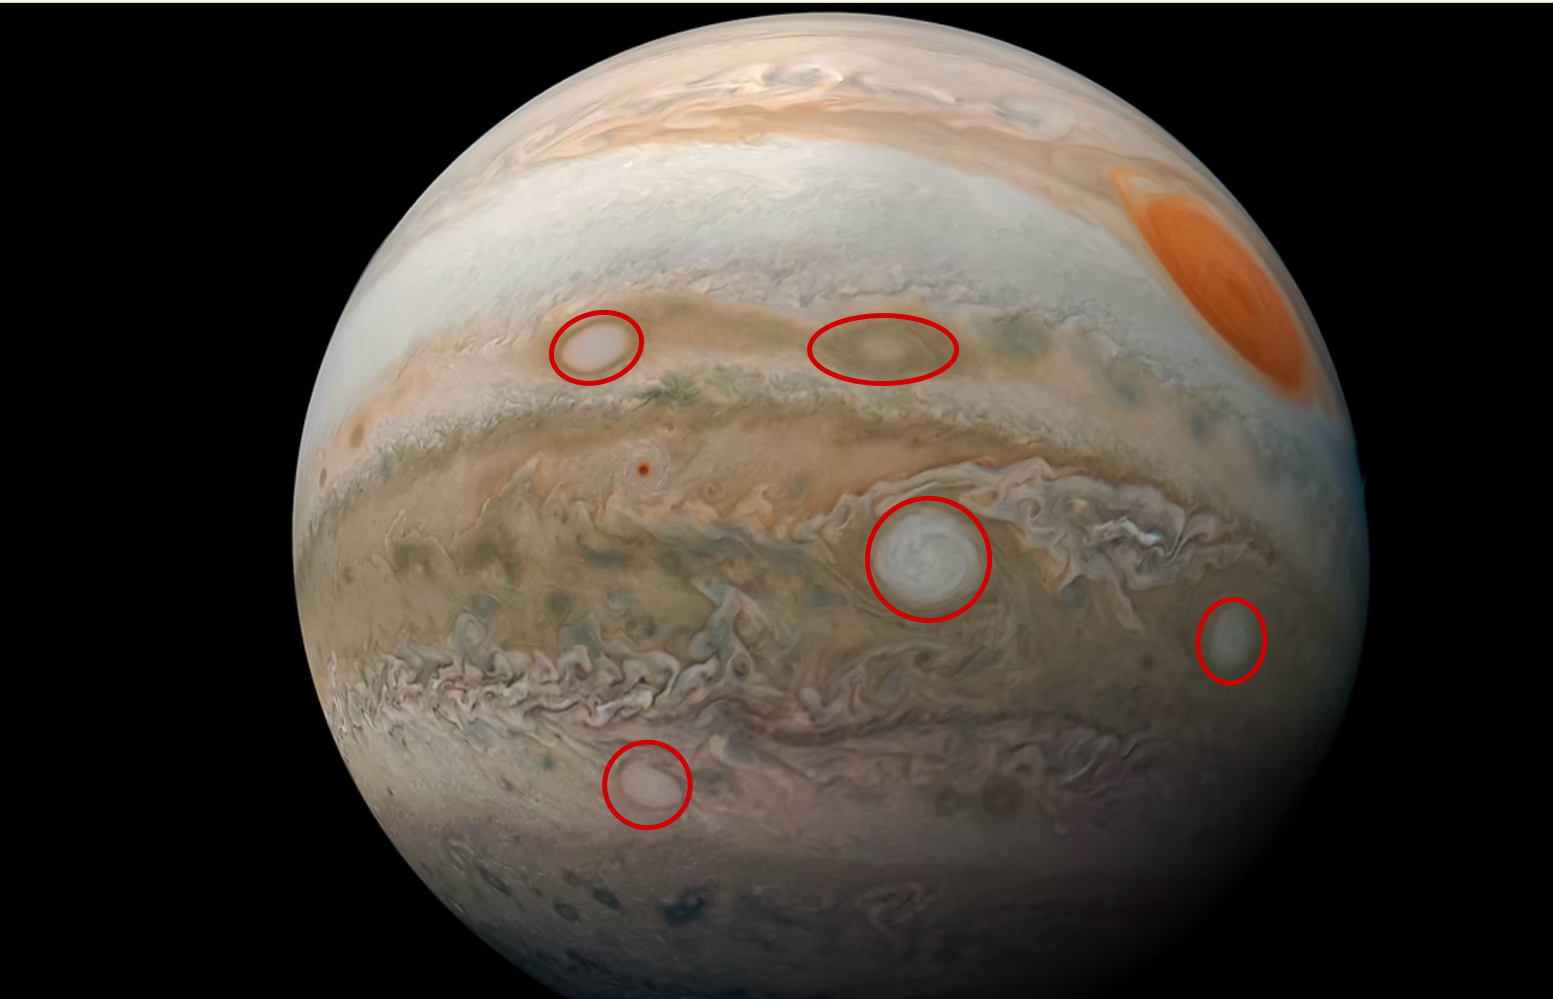
\includegraphics[width=0.95\linewidth]{slike/vrtinci.jpeg}
    %\caption{A subfigure}
    %\label{fig:sub1}
  \end{subfigure}%
  \begin{subfigure}{.5\textwidth}
    \centering
    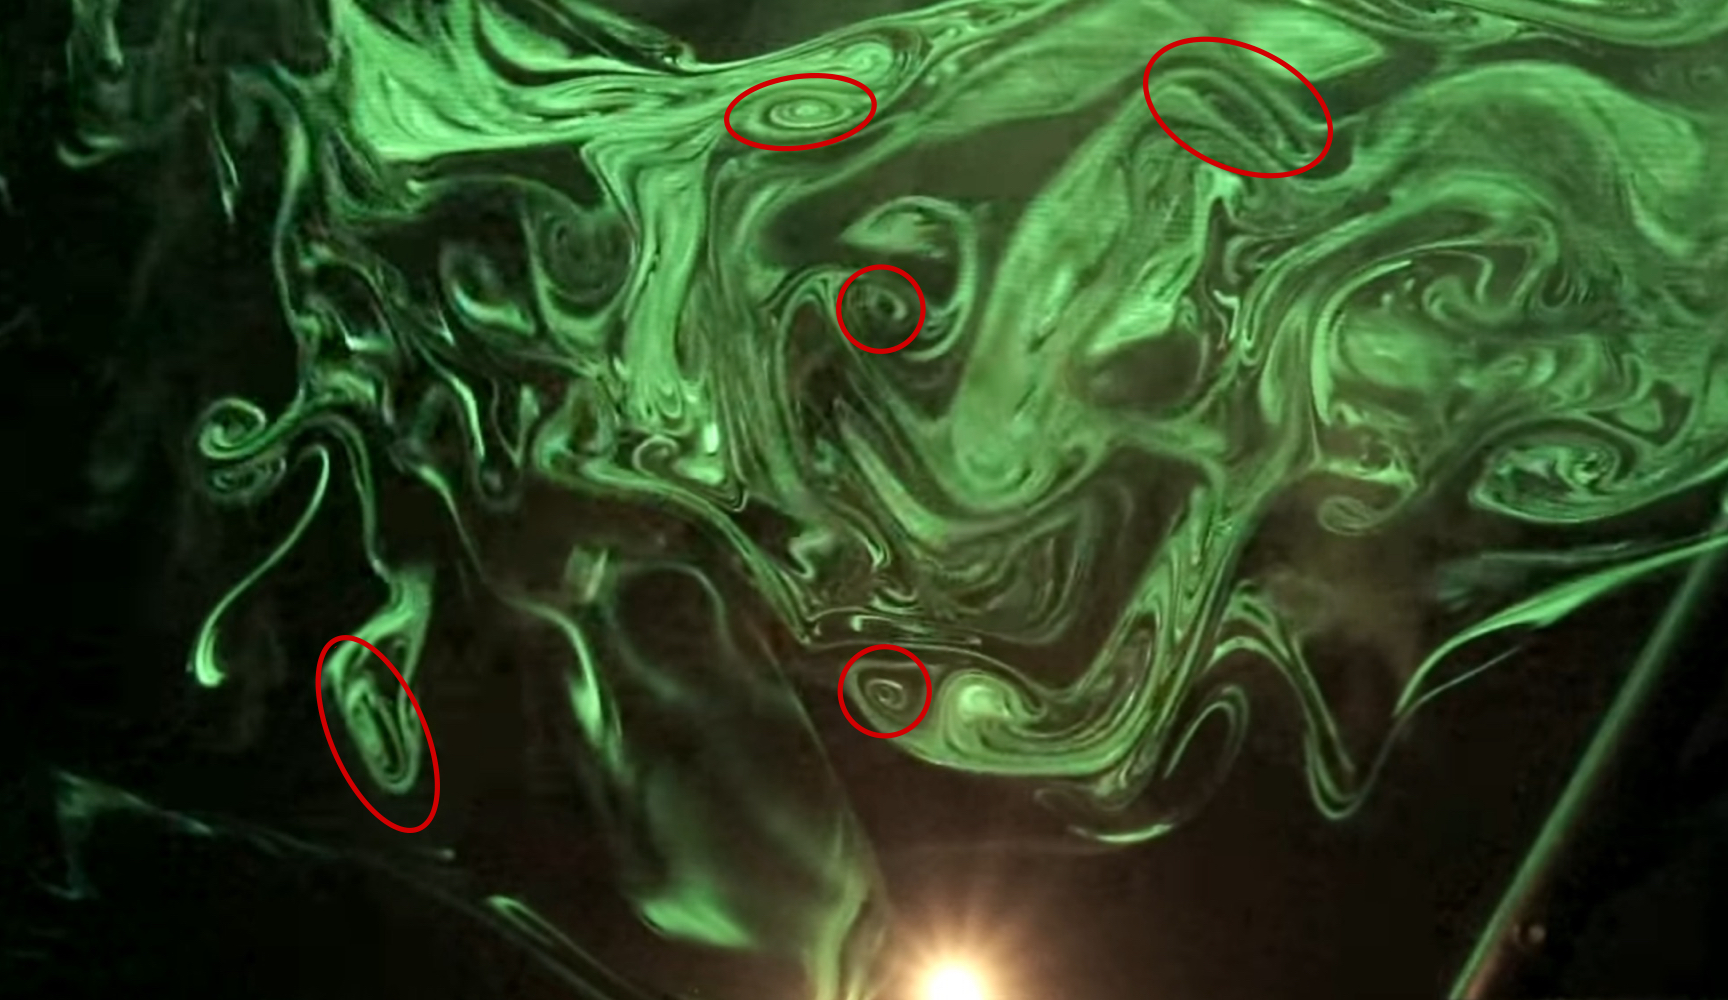
\includegraphics[height=4.58cm, width=0.95\linewidth]{slike/vrtinci2.jpeg}
    %\caption{A subfigure}
    %\label{fig:sub2}
  \end{subfigure}
  \caption{Leva slika prikazuje velike vrtince, ki se pojavijo v atmosferi planeta Jupitra in 
  imajo lahko premer dolžine več $1000$ kilometrov, med tem ko desna slika prikazuje turbulenco
  zraka v sobi, kjer se tok zraka prikaže s pomočjo laserja in lahko vidimo vrtince velikosti nekaj mikrometrov} 
  \label{fig:vrtinci}
  \end{figure}
\item \textbf{Difuzivnost}: Zanimiva lastnost turbuletnega toka je difuzivnost. To poemni, da se energija in gibalna količina
preneseta po celotnem toku. Osborne Reynolds (1842 - 1912) je postavil eksperiment, ki prikazuje to lastnost. Vidno je
na sliki \ref{fig:difus}
\item \textbf{Reynoldsovo število}: Podoben eksperiment kot pri sliki \ref{fig:difus} nam da enostaven kriterij, ki mu turbulenca zadošča.
Večja kot je dolžina cevi $L$ ali večja kot je hitrost toka $u$ prej bo prišlo do turbulence. Po drugi strani pa večja kot je
viskoznost tekočine, manj verjetno bo, da pride do turbulence. To zapišemo kot kot brez dimenzijsko 
konstanto $Re = \frac{uL}{\nu}$. Do turbulence pride pri velikih Reynoldsovih številih, običajno $Re \geq 5000$.
\item \textbf{Disipativnost}: To je proces prenosa energije iz večjih vrtincev v najmanjše vrtince, dokler ta ne 
začne izhajati iz tekočine kot toplota. To pomeni, če hočemo imeti turbulenten tok oz. ga ohranjati
moramo dosledno dodajati energijo sistemu.
\begin{figure}[h!]
  \centering
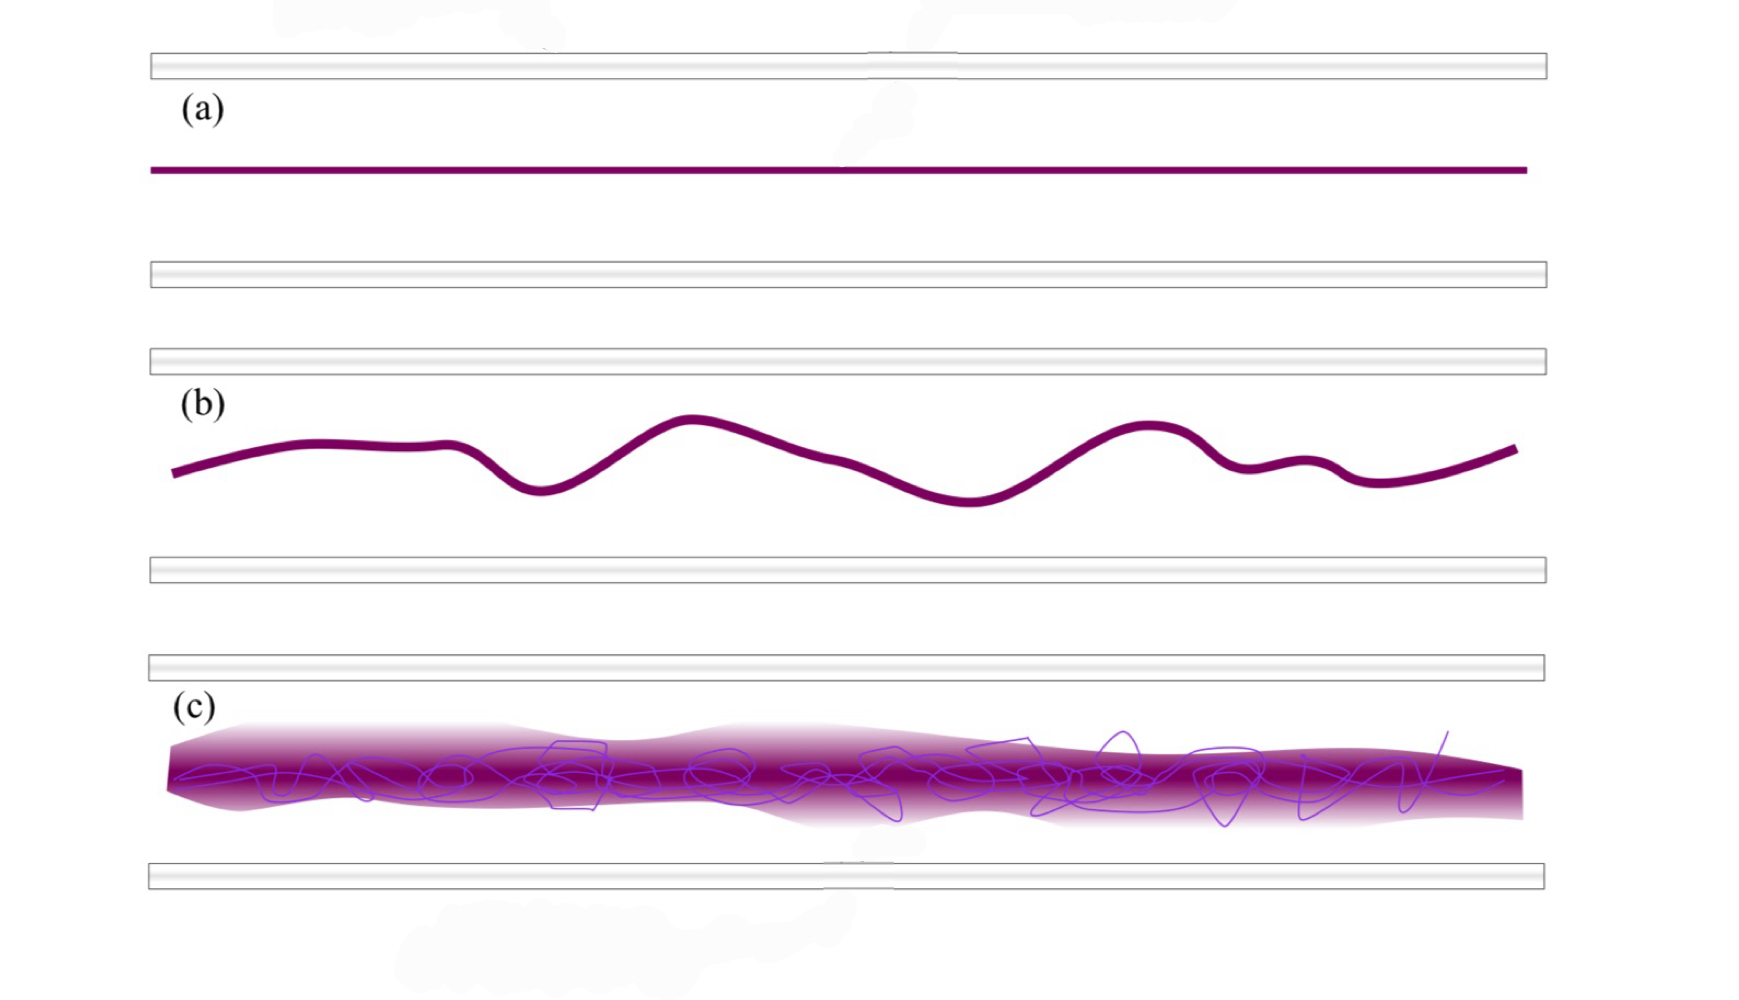
\includegraphics[scale=0.19]{slike/difus.jpeg}
\caption{V cev s polno vode, spustimo tok barve. Slika je sestavljena iz treh delov, a) del ni turbulenten zato se barva zalo malo razprši,
b) del je v vmesnem stanju, kjer se že kažejo znaki difuzije in c) del kjer se tok turbulenten in se barva razširi po celotni cevi.}
\label{fig:difus}
\end{figure}
\begin{figure}[h]
  \centering
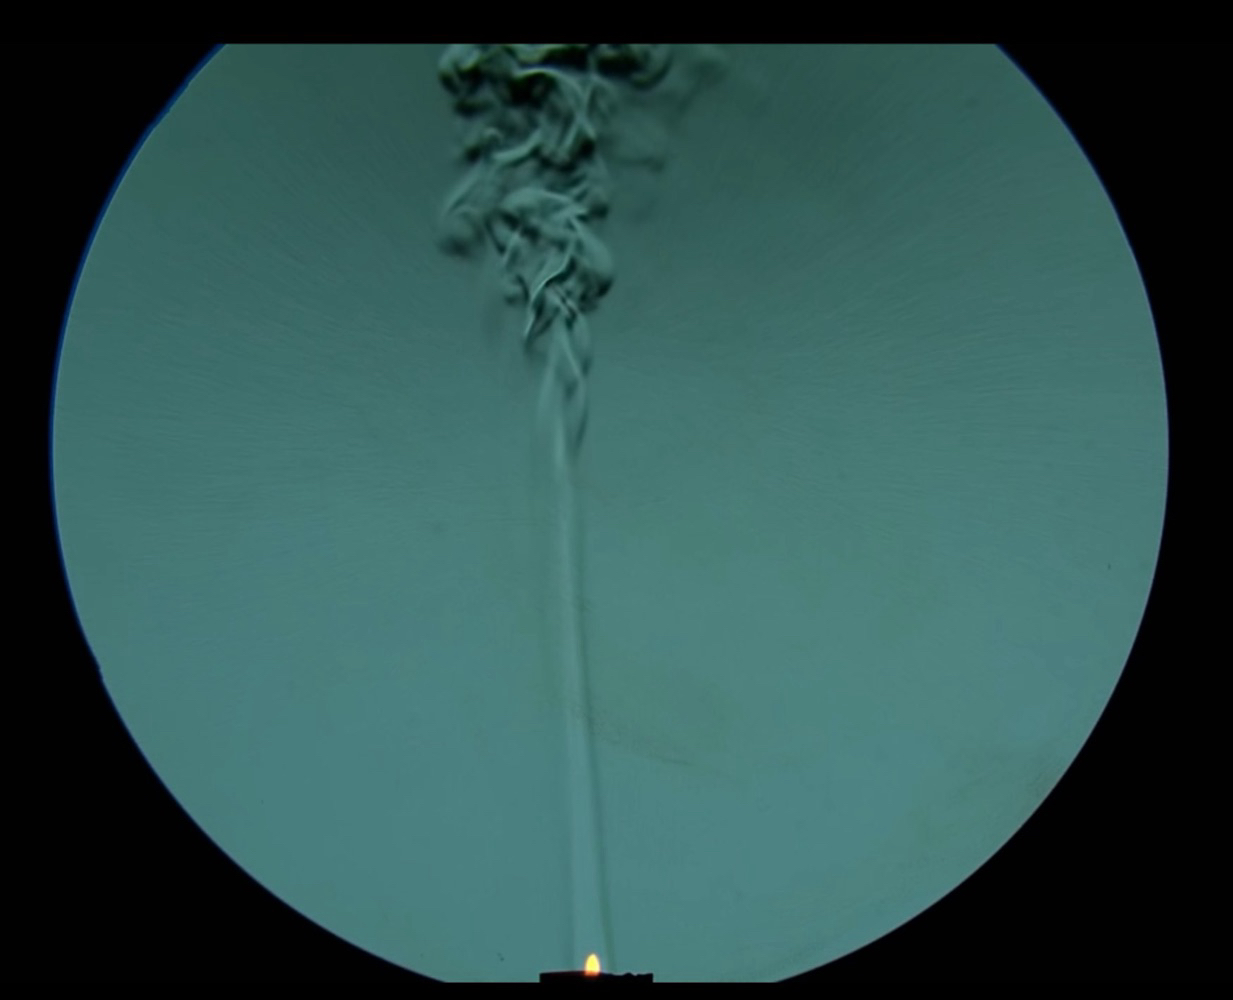
\includegraphics[scale=0.19]{slike/Reynolds.jpeg}
\caption{Slika prikazuje hlape plamena, kako se potujejo v zraku. Na začetku, kjer imamo majhno Reynoldsovo število je tok zelo predvidljiv,
ko pa se dviguje (parameter $L$ se veča) se Reynoldsovo število veča in tok postane turbulenten.}
\end{figure}
\end{itemize}

V delu se bom predvsem osredotočil na turbulenco v atmosferi, kjer je obravnava določenih enačb
gibanja in fizikalnih količin obravanava nekoliko drugače, kot pri drugih vrstah turbulence (kot so naprimer turbulence tekočin).
V splošnem pa se kakršen koli tok obravanava na enega od sledečih načinov:
\begin{itemize}
  \item \textbf{Eulerjev pristop}: recimo, da opazujemo neko domeno $D$ skozi katero teče tok.
  Zanima nas hitrost $u(x, t)$ za $x \in D$ ob času $t > 0$. V tem primeru smo fiksirali koordinatni
  sistem (glede na zemljo).
  \item \textbf{Lagrangeev pristop}: pri tem pristopu opazujemo s kakšno hitrostjo se delec toka 
  $x$ premika skozi čas. Označimo $u(t; x_0)$, kjer je $x_0$ začetna pozicija delca in 
  $u$ hitrost delca ob času $t$. 
\end{itemize}

Kateri pristop uporabimo je odvisno lastnost, ki jih želimo analizirati. Eulerjev pristop
se osredotoči na fiksno domeno in opazujemo kako se lastnosti tekočine spreminjajo v tej skozi čas. 
Za analizo turbulence in globalnih procesov je ta način boljši, med tem ko analiza po 
Lagrage-u boljša za analizo mehanike delcev, disperzije in različnih procesov mešanja (difuzija). 

V delu bomo primarno uporabljali Eulerjev-jev pristop, vendar pa nam analiza enega pomaga
lahko pri analizi drugega. Naj bo $u$ Eulerjevo polje hitrosti na poljubni domeni. Po Lagrangeevem 
opisu, delec toka ob času $t$ in začeti pozicija $y_0$ ob času $t_0$ označimo z $X(t, y_0)$.
Pozicija delca je podana z enačbama
\begin{align}
&X(t_0, y_0) = y_0 \\
\frac{\partial}{\partial t} X&(t, y_0) = u(X(t, y_0), t)
\end{align}
Definiramo Langrageovo polje hitrosti
\begin{equation}
U(t, y_0) = u(X(t, y_0), t).
\end{equation}
Poglejmo kako se izraža pospešek delca
\begin{align*}
\frac{\partial }{\partial t} U(t, y_0) &= \frac{\partial}{\partial t} u(X(t, y_0), t) = \\
&= \Big(\frac{\partial}{\partial t} u(x, t) \Big)_{x = X(t, y_0)} + \frac{\partial}{\partial t} X(t, y_0) \cdot \Big(\text{grad}_x u(x, t) \Big)_{x = X(t, y_0)} = \\
&= \Big(\frac{\partial}{\partial t} u(x, t) + u(t, y_0) \cdot \text{grad}_x u(x, t) \Big)_{x = X(t, y_0)} = \\
&= \Big(\frac{D}{Dt} u(x, t) \Big)_{x = X(t, y_0)}
\end{align*}
\begin{definicija}
Naj bo $U$ poljubno vektorsko polje. Diferencialni operator 
\begin{equation}
\frac{D}{Dt} = \frac{\partial}{\partial t} + U \cdot \nabla
\end{equation}
se imenuje materialni odvod.
\end{definicija}

Podoben rezultat dobimo, če namesto hitrosti, odvajamo gostoto
$$
\frac{\partial }{\partial t} \mathrm{P}(t, y_0) = \Big(\frac{D}{Dt} \rho(x, t) \Big)_{x = X(t, y_0)}.
$$
Materialni odvod je fundementalni operator Eulerjevaga pristopa. Vedno, ko nas bo 
zanimalo kako se neka količina spreminja s časom, nas bo zanimal njen materialni odvod.

\begin{opomba}
Operator $\nabla$ ni komutativen: $U \cdot \nabla \neq \nabla \cdot U$.
\end{opomba}


\subsection{Ohranitveni zakoni}

S tem razdelkom začnemo matematični opis enega najbolj pomembnih konceptov iz dinamike fluidov (in fizike na splošno), 
ki so ključni za razumevanje turbulentnih tokov. 

\begin{opomba}
V nadaljevanju bomo izpeljali formule, brez da bi (vsakič) navedli vseh nujnih predpostavk. Na primer 
običajno bodo domene s katerimi imamo opravka gladke orientabilne mnogoterosti ali vektorsko polje
$u$, ki bo običajnoi gladko, zato da bomo lahko uporabili Stokesov izrek.
\end{opomba}

\subsubsection{Zakon o ohranitvi mase}
Naj bo $\Delta \subseteq R^3$ omejena, $\partial \Delta$ njen rob in $\rho: \Omega \times [0, \infty] \rightarrow [0, \infty]$ 
gostota množice $\Omega$, ki je gladka. Masa $m$ od $\Omega$ je 
$$
m = \int_\Omega \rho(x, t) \dif\Omega.
$$
\begin{center}
\begin{tikzpicture}
  \draw  plot[smooth, tension=.7] coordinates {(-3.5,0.5) (-3,2.5) (-1,3.5) (1.5,3) (4,3.5) (5,2.5) (5,0.5) (2.5,-2) (0,-0.5) (-3,-2) (-3.5,0.5)};
  \draw[thick, rotate = 30] (-1.3,0.8) ellipse (0.4 and 0.7);
  \filldraw[red, rotate = 30] (-1.3,0.8) circle(2pt) ;
  \draw[thick, red, rotate = 30, ->] (-1.3,0.8) -- (-3,0.7) node[above, black] {$\mathbf{\vec{u}}$};
  \node at (1.5,1.5) {$\Omega$};
  \node at (4,4) {$\partial$$\Omega$};
\end{tikzpicture}
\end{center}
~\\[1mm]

Zakon o ohraniti mase pravi, da je količina mase, ki se pretoči v $\Omega$ v določenem času, 
enaka količini mase, ki se iztoči skozi $\partial\Omega$ tj.
$$
\frac{\partial m}{\partial t} = - \int_{\partial \Omega} \rho \dif \vec{S}.
$$
Ker je normala na $\partial \Omega$ dana z $\vec{u}$, lahko zakon zapišemo kot 
$$
\int_\Omega \frac{\partial}{\partial t} \rho(x, t) \dif V = - \int_{\partial \Omega} \rho \vec{u} \dif S.
$$
Če uporabimo izrek o divergenci, velja:
$$
\int_{\partial \Omega} \rho\vec{u} \dif \vec{S} = \int_{\Omega} \nabla \cdot \rho\vec{u} \dif V
$$
Dobimo 
\begin{align*}
\int_\Omega \frac{\partial}{\partial t} \rho(x, t) + \nabla \cdot (\rho\vec{u}) \dif V = 0
\end{align*}
Ker enakost velja za vsako domeno $\Omega$ je
\begin{equation}
\frac{\partial \rho}{\partial t} + \nabla \cdot (\rho\vec{u}) = 0.
\end{equation}

(Ali dodam dokaz te lastnosti?)\\
To je diferencialna oblika zakona o ohraniti mase in tej enačbi pravimo \textbf{kontinuitetna enačba}.
Če je gostota konstantna, tj $\rho(x, t) \equiv c > 0$, potem se kontinuitetna enačba poenostavi
$$
\frac{\partial \rho}{\partial t} + \nabla \cdot (\rho\vec{u}) = \rho \nabla u = 0 \Longrightarrow \nabla u = 0.
$$
\begin{definicija}
Tok je \textbf{nestisljiv}, če velja 
\begin{equation}
\label{ohranitev mase}
  \nabla u = 0.    
\end{equation}
\end{definicija}

\subsection{Zakon o ohranitvi gibalne količine}
V tem razdelku bomo predpostavili, da je gostota $\rho$ konstantna, tj.
\begin{equation}
m = \int_\Omega \rho \dif V = \rho \int_\Omega \dif V = \rho \cdot V,
\end{equation}
kjer je $V = \int_\Omega \dif V$ volumen domene $D$. Zakon o ohranitvi gibalne količine, 
pravi, da je vsota gibalnih količin ($p$) v zaprtem sistemu konstanten. Če imamo $n$ delcev je
\begin{align*}
&\sum_{k=1}^n p_k = \text{const.} \\[1mm]
&\sum_{k=1}^n \frac{\dif p_k}{\dif t} = 0.
\end{align*}
Ker je gibalna količina $p = m v$, lahko ekvivalentno zapišemo
\begin{align*}
\frac{\dif p}{\dif t} = \frac{\dif \,(m v)}{\dif t} &= m\frac{\dif v}{\dif t} = m a = F \Longrightarrow\\[2mm]
\sum_{k=1}^n F_k &= 0.
\end{align*}
To je ravno 1. Newtonov zakon, če upoštevamo še 2. Newtonov zakon:
\begin{equation}
\sum_{k=1}^n F_k = m a.
\end{equation}
Zapišimo ta zakon za tokove
\begin{align*}
m a = \rho V \frac{D u}{D t} = \sum_{k=1}^n F_k \\
\rho \frac{D u}{D t} = \sum_{k=1}^n \frac{F_k}{V}. 
\end{align*}
Pri tokovih se pojavita dve vrsti sil 
\begin{itemize}
  \item Ploskovne sile, ki jih delimo na 
  \begin{enumerate}
    \item[1)] Tangencialne (viskoznost)
    \item[2)] Normalne (tlak)
  \end{enumerate}
  \item Telesne oz. zunanje sile (gravitacija, Corioliosva sila, magnetizem, \dots)
\end{itemize}
Sedaj bomo te zapisali s hitrostjo toka $u$, da dobimo enačbo, ki opisuje gibanje le tega.\\
\textbf{Normalna sila .oz tlak:}\\[1mm]
\begin{center}

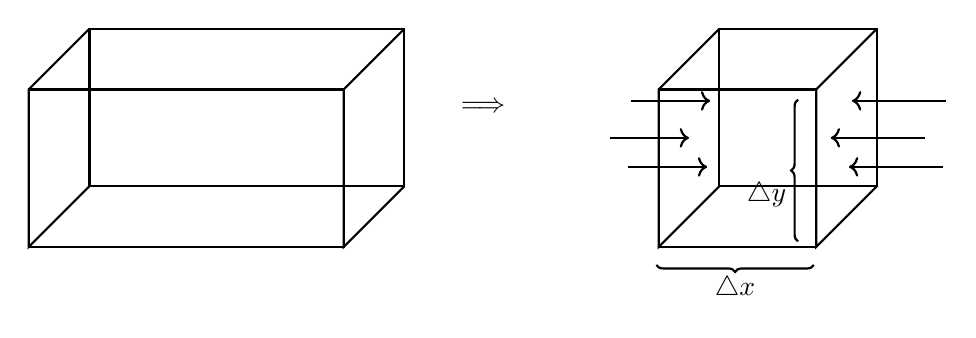
\begin{tikzpicture}[scale=2]
  \draw[thick] (-4,0,0) -- (-2,0,0) -- (-2,1,0) -- (-4,1,0) -- cycle; % Bottom face
  \draw[thick] (-4,0,0) -- (-4,0,1) -- (-4,1,1) -- (-4,1,0);          % Left face
  \draw[thick] (-2,0,0) -- (-2,0,1) -- (-2,1,1) -- (-2,1,0);          % Right face
  \draw[thick] (-4,0,1) -- (-2,0,1) -- (-2,1,1) -- (-4,1,1) -- cycle; % Top face

  \draw[thick] (0,0,0) -- (1,0,0) -- (1,1,0) -- (0,1,0) -- cycle; % Bottom face
  \draw[thick] (0,0,0) -- (0,0,1) -- (0,1,1) -- (0,1,0);          % Left face
  \draw[thick] (1,0,0) -- (1,0,1) -- (1,1,1) -- (1,1,0);          % Right face
  \draw[thick] (0,0,1) -- (1,0,1) -- (1,1,1) -- (0,1,1) -- cycle; % Top face

  % Left arrow
  \draw[->, thick] (-0.5, 0.2, 0.2) -- (0, 0.2, 0.2);
  \draw[->, thick] (-0.5, 0.5, 0.5) -- (0, 0.5, 0.5);
  \draw[->, thick] (-0.5, 0.6, 0.15) -- (0, 0.6, 0.15);

  % Right arrow
  \draw[->, thick] (1.5, 0.2, 0.2) -- (0.9, 0.2, 0.2);
  \draw[->, thick] (1.5, 0.5, 0.5) -- (0.9, 0.5, 0.5);
  \draw[->, thick] (1.5, 0.6, 0.15) -- (0.9, 0.6, 0.15);

  %\draw[->, thick] (0.9, 1.9, 1.5) -- (0.9, 1.4, 1.5);
  %\draw[->, thick] (1.2, 1.9, 1.7) -- (1.2, 1.4, 1.7);
  %\draw[->, thick] (0.6, 1.9, 1.7) -- (0.6, 1.4, 1.7);

  \node at (-1.5, 0.5, 0) {$\Longrightarrow$};
  %\node at (0.5, -0.5, 0) {Front};
  \draw[thick, decorate, decoration={brace, mirror}] (-0.4, -0.5, 0) -- (0.6, -0.5, 0) 
        node[midway, yshift=-0.3cm] {$\triangle x$};
  \draw[thick, decorate, decoration={brace}] (0.5, -0.35, 0) -- (0.5, 0.55, 0) 
        node[midway, xshift = -0.4cm, yshift=-0.3cm] {$\triangle y$};
\end{tikzpicture}
\end{center}

Recimo, da imamo majhno domeno $\Omega$ z volumnom $V = \triangle x \triangle y  \triangle z$.
Poglejmo. kako se sila izraža v $x$ - smeri, če pridedo sprememe tlaka. Ta je definiran kot $p = \frac{\triangle F}{\triangle A}$, 
kjer sta $\triangle F$ - majhna sprememba sile in $\triangle A$ - majhna sprememba površine. Imamo:
\begin{align*}
F_x &= p_1 A_1 - p_2 A_2 = \quad \quad(A_1 = A_2 = A) \\
F_x &= (p_1 - p_2)A = \triangle p A \quad \Longrightarrow \\
\frac{F_x}{V} &= \frac{\triangle p \triangle y \triangle z}{\triangle x \triangle y \triangle z} = \frac{\triangle p}{\triangle x}
\end{align*}
Pošljemo $\triangle x$ proti $0$:
$$
\frac{F}{V} = \lim_{\triangle x \rightarrow 0 }\frac{F_x}{V} = \lim_{\triangle x \rightarrow 0} \frac{\triangle p}{\triangle x} = \frac{\partial p}{\partial x}
$$
Na enak način dobimo v smereh $y$ in $z$.

\noindent
\textbf{Tangencialna sila oz. viskoznost:} \\[1mm]
Viskoznost ima podobno vlogo kot trenje. To je namreč sila med dvema tokovoma različnih
hitrosti. Te količini pravimo strižna napetost, ki je definirana enako kot tlak, vendar kaže v drugo smer, $\tau = \frac{F}{A}$. \\[2mm]
\begin{center}
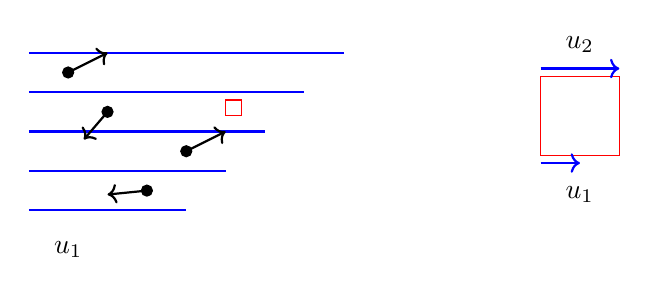
\begin{tikzpicture}
  % Draw horizontal blue lines of different lengths
  \draw[thick, blue] (0,2) -- (4,2);
  \draw[thick, blue] (0,1.5) -- (3.5,1.5);
  \draw[thick, blue] (0,1) -- (3,1);
  \draw[thick, blue] (0,0.5) -- (2.5,0.5);
  \draw[thick, blue] (0,0) -- (2,0);
  
  % Add atoms as small circles
  \filldraw[black] (1.5,0.25) circle(2pt) node[below] {};
  \filldraw[black] (2,0.75) circle(2pt) node[below] {};
  \filldraw[black] (1,1.25) circle(2pt) node[below] {};
  \filldraw[black] (0.5,1.75) circle(2pt) node[below] {};
  
  % Add arrows for the motion of atoms
  \draw[->, thick] (1.5,0.25) -- (1,0.2);
  \draw[->, thick] (2,0.75) -- (2.5,1);
  \draw[->, thick] (1,1.25) -- (0.7,0.9);
  \draw[->, thick] (0.5,1.75) -- (1,2);
  
  % Add a small red square
  \draw[red] (2.5,1.2) rectangle +(0.2,0.2);
  
  
  \draw[red] (6.5,0.7) rectangle +(1,1);
  \draw[->, thick, blue] (6.5,0.6) -- (7,0.6);
  \draw[->, thick, blue] (6.5,1.8) -- (7.5,1.8);
  \node at (0.5, -0.5, 0) {$u_1$};

  % Add labels
  \node at (7.3,2.1) [left] {$u_2$};
  \node at (7.3,0.2) [left] {$u_1$};
\end{tikzpicture}
\end{center}
Če gledamo spremembo hitrosti v $x$ - smeri
$$
\tau_x = \frac{F_x}{A} = \frac{m}{A} \cdot \frac{\triangle u}{\triangle t}\cdot \frac{\triangle y}{\triangle y} = \underbrace{\frac{m}{A} \cdot\frac{\triangle y}{\triangle t}}_{\mu} \cdot\frac{\triangle u}{\triangle y} = \mu \frac{\triangle u}{\triangle y}
$$
$\tau_x$ je dinamična viskoznost in odvisna od lastnosti tekočine. 
Ko pošljemo $\triangle y \rightarrow 0$, dobimo
$$
\tau = \lim_{\triangle y \rightarrow 0} \tau_x = \lim_{\triangle y \rightarrow 0} \frac{\triangle u}{\triangle y} = \frac{\partial u}{\partial y}
$$
Naredimo podobno analizo, kot pri tlaku \\
\begin{center}
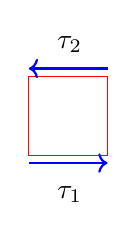
\begin{tikzpicture}
  \draw[red] (3.5,0.7) rectangle +(1,1);
  \draw[->, thick, blue] (3.5,0.6) -- (4.5,0.6);
  \draw[->, thick, blue] (4.5,1.8) -- (3.5,1.8);

  % Add labels
  \node at (4.3,2.1) [left] {$\tau_2$};
  \node at (4.3,0.2) [left] {$\tau_1$};
\end{tikzpicture}
\end{center}
Če sta strižni napetosti različni, imamo neničelni silo na majhnem območju $\Omega = \triangle x \triangle y \triangle z$:
\begin{align*}
F_x &= \tau_2 A_2 - \tau_1 A_1  \quad (A_1 = A_2)\\
F_x &= \triangle \tau \triangle x \triangle z  \quad \Longrightarrow\\
\frac{F_x}{V} &= \frac{\triangle \tau \triangle x \triangle z}{\triangle x \triangle y \triangle z} = \frac{\triangle \tau}{\triangle y}.
\end{align*}
Ponovno pošljemo $\triangle y \rightarrow 0$
$$
\frac{F}{V} = \lim_{\triangle y \rightarrow 0} \frac{F_x}{V} = \lim_{\triangle y \rightarrow 0} \frac{\triangle \tau}{\triangle y} = \frac{\partial \tau}{\partial y} = \frac{\partial}{\partial y} \Big(\frac{\mu\partial u}{\partial y} \Big) = \mu \frac{\partial^2 u}{\partial y^2}.
$$
Strižno napetost upoštevamo v vseh treh smereh, je
$$
\frac{F}{V} = \mu \Big(\frac{\partial^2 u}{\partial x^2} + \frac{\partial^2 u}{\partial y^2} + \frac{\partial^2 u}{\partial z^2}  \Big)
$$
(Zakaj točno so tu odvodi v vseh treh smereh, ne pa pri tlaku?) \\[1mm]
\textbf{Telesne sile:} \\
V splošnem je tukaj lahko veliko različnih sil, tu pa bomo upoštevali le gravitacijo (ko bomo začeli z modeliranjem atmosfere, bo ključno, da upoštevamo še Corioliosovo silo). Gravitacijska sila v primeru tokov 
$$
\frac{F}{V} = \frac{m g}{V} = \frac{\rho V g}{V} = \rho g.
$$
Ko združimo vse tri sile, dobimo enačbo
$$
\rho \frac{D u}{D t} = - \frac{\partial p}{\partial x} + \mu \Big( \frac{\partial^2 u}{\partial x^2} + \frac{\partial^2 u}{\partial y^2} + \frac{\partial^2 u}{\partial z^2} \Big) + \rho g.
$$
Če upoštevamo, da je hitrost vektorsko polje, imamo tri komponente hitrosti, zato $3$ enačbe 
\begin{align*}
  \rho \frac{D u}{D t} &= - \frac{\partial p}{\partial x} + \mu \Big( \frac{\partial^2 u}{\partial x^2} + \frac{\partial^2 u}{\partial y^2} + \frac{\partial^2 u}{\partial z^2} \Big) + \rho g_x \\
  \rho \frac{D v}{D t} &= - \frac{\partial p}{\partial y} + \mu \Big( \frac{\partial^2 v}{\partial x^2} + \frac{\partial^2 v}{\partial y^2} + \frac{\partial^2 v}{\partial z^2} \Big) + \rho_y g\\
  \rho \frac{D w}{D t} &= - \frac{\partial p}{\partial z} + \mu \Big( \frac{\partial^2 w}{\partial x^2} + \frac{\partial^2 w}{\partial y^2} + \frac{\partial^2 w}{\partial z^2} \Big) + \rho g_z
\end{align*}
Kompaktno lahko zapišemo 
$$
\rho \frac{D U}{D t} = - \nabla p + \mu \nabla^2 U + \rho g,
$$
kjer je $U = (u, v, w)$ in $g = (g_x, g_y, g_z)$. Tem enačbam pravimo Navier-Stokesove enačbe.
Običajno se zadnjo enačbo deli z gostoto $\rho$ in uvede \textbf{kinematično viskoznost}
$\nu = \frac{\mu}{\rho}$. V nadaljevanju bomo uporabljali $u$ za vektor hitrosti in se enačba
glasi
\begin{equation}
  \label{NS}
\frac{D u}{D t} = \frac{\partial u}{\partial t} + (u\cdot \nabla)u = - \frac{1}{\rho}\nabla p + \nu \nabla^2 u + \rho g.
\end{equation}

\begin{opomba}
  \hfil
\begin{itemize}
  \item Če ne poznamo telesnih sil ali jih imamo več, v zadnji enačbi sumand zamenjamo z $f$.
  \item Količine deljene z gostoto, imenujemo kinematiče količine.
\end{itemize}
\end{opomba}

\subsection{Zakon o ohranitvi vrtinčnosti}

Omenimo še količino vrtinčenja. Kot že ime pove, je to količina, ki opisuje vrtenje toka okoli neke točke. 
\begin{definicija}
Naj bo $u$ vektor hitrosti. Vrtinčenje $\omega$ je rotor polja $u$
\begin{equation}
\omega \equiv \nabla \times u.
\end{equation}
\end{definicija}
Ohranitveno enačbo za $\omega$ dobimo preko Navier-Stokesove enačbe. Predpostavimo, 
da je vektorsko polje $u \in C^2$ na poljubni domeni. Vzamemo rotor enačbe \eqref{NS}:
\begin{align*}
\nabla \times (\frac{\partial u}{\partial t} + (u\cdot \nabla)u) = \nabla\times (- \frac{1}{\rho}\nabla p + \nu \nabla^2 u + f) \\
\frac{\partial \omega}{\partial t} + \nabla \times ((u\cdot \nabla)u) = - \frac{1}{\rho} \nabla \times (\nabla p) + \nu\nabla^2 \omega + \nabla \times f
\end{align*}
Dobro znano dejstvo je, da je rotor gradienta skalarne funkcije $0$, torej je 
$\nabla \times (\nabla p) = 0$. Poenostavimo člen s hitrostjo. Iz dvojnega vektorskega 
produkta dobimo 
\begin{align*}
u \times (\nabla \times u) &=  \nabla(u\cdot u) - (u\cdot \nabla)u \\
\Longrightarrow \quad(u\cdot \nabla)u &= \nabla (u\cdot u) - u\times (\underbrace{\nabla \times u}_{= \omega})
\end{align*}
Vzamemo rotor zadnje enakosti:
\begin{align*}
\nabla \times (u\cdot \nabla)u &= \underbrace{\nabla \times (\nabla(u\cdot u))}_{= 0} - \nabla \times (u \times \omega) \\
&= \nabla \times (\omega \times u) \\
&= (u\cdot \nabla)\omega - (\omega \cdot \nabla)u + \omega\underbrace{(\nabla \cdot u)}_{= 0 \text{ po } \eqref{ohranitev mase}} + u \underbrace{(\nabla \cdot \omega)}_{= 0}
\end{align*}
Vstavimo v prvotno enačbo
\begin{align*}
\frac{\partial \omega}{\partial t} + (u\cdot \nabla)\omega + (\omega \cdot \nabla)u - (\omega \cdot \nabla)u + u (\nabla \cdot \omega) =  \nu\nabla^2 \omega + \nabla \times f
\end{align*}
Enačba, ki nam zakaon opiše 
\begin{equation}
\frac{D\omega}{D t} = \frac{\partial \omega}{\partial t} + (u\cdot \nabla)\omega = (\omega \cdot \nabla)u+ \nu \nabla^2 \omega + \nabla \times f.
\end{equation}

\subsection{Zakon o ohranitvi skalarja}
Sedaj bomo posplošili zakon o ohranitvi mase, za poljubno zvezno odvedljivo skalarno polje $c: \R\times \R^3 \rightarrow \R$.
Začnemo z enako enačbo kot pri zakonu o ohranitvi mase, le, da dodamo še dva dodatna 
člena. Ta člena sta $F$ - vektorsko polje, za pretok oz. prenos skalarja $c$ in $H$ - izvor za skalar $c$.
V integralski obliki dobimo zapis:
\begin{equation}
\frac{\dif}{\dif t} \int_{\Omega} c \dif V = - \int_S \vec{F} \cdot \dif \vec{S} - 
\int_S c \vec{u}  \dif \vec{S} + \int_\Omega H \dif V,
\end{equation}
kjer je $\Omega$ omejena domena in $S = \partial \Omega$.
Prva dva člena imata negativen predznak, ker skalar odteka. Če je $H < 0$ potem 
imamo oddtok skalarja, če pa je $H > 0$ imamo pritok skalarja. 

\begin{primer}
Enostaven primer, ki pokaže pomen količine $H$. Pri zgornji luknji imamo pritok 
mase (tekočine) in v tem primeru je $H_{p} > 0$, med tem ko imamo v spodnji luknji oddtok
mase (tekočine) in je $H_{0} > 0$. Celotni $H$ lahko zapišemo kot $H = H_p - H_0$.
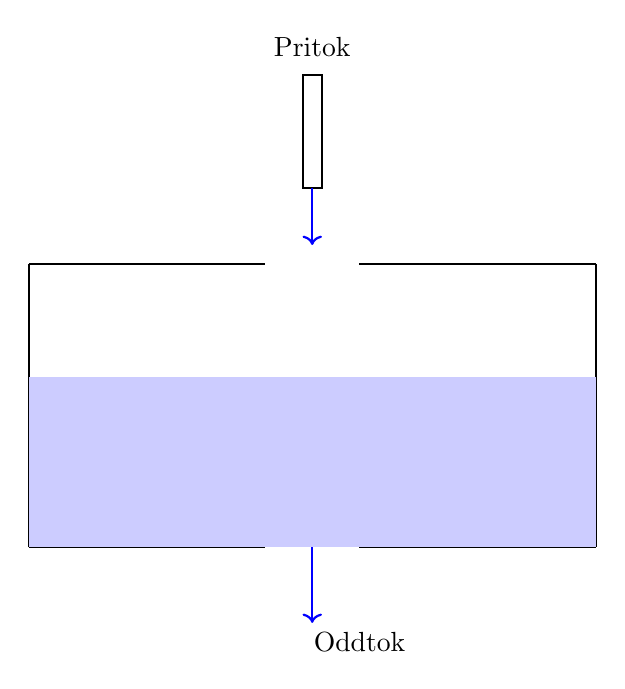
\begin{tikzpicture}[scale=1.2]

  % Basin (korito) with gaps at the bottom and top
  \draw[thick] (0,0) -- (2.5,0);    % Left part of bottom line
  \draw[thick] (3.5,0) -- (6,0);    % Right part of bottom line
  
  \draw[thick] (0,3) -- (2.5,3);    % Left part of top line
  \draw[thick] (3.5,3) -- (6,3);    % Right part of top line
  
  \draw[thick] (0,0) -- (0,3);      % Left wall
  \draw[thick] (6,0) -- (6,3);      % Right wall
  
  % Water level inside basin
  \fill[blue!20] (0,0) rectangle (6,1.8);
  
  % Narrow inflow pipe (higher up)
  \draw[thick] (2.9,5) rectangle (3.1,3.8);
  
  % Water inflow stream
  \draw[blue, thick, ->] (3,3.8) -- (3,3.2);
  
  % Outflow stream at bottom hole
  \draw[blue, thick, ->] (3,0) -- (3,-0.8);
  
  % Outflow stream at top hole
  %\draw[blue, thick, ->] (3,3) -- (3,3.5);
  
  % Labels
  \node at (3,5.3) {Pritok};
  \node at (3.5,-1) {Oddtok};
  %\node at (3.9,3.5) {Top outflow};
  
  % H explanation
  %\node at (7,2.2) {\Large $H = \text{Inflow} - \text{Outflows}$};
\end{tikzpicture}
\end{primer}
Zapišemo diferencialno enačbo za zgornjo integralsko enačbo. Po Stokesovem izreku:
\begin{align*}
\frac{\dif}{\dif t} \int_{\Omega} c \dif V &= - \int_S \vec{F} \cdot \dif \vec{S} - 
\int_S c \vec{u}  \dif \vec{S} + \int_\Omega H \dif V \\
\int_{\Omega} \frac{\partial c}{\partial t} \dif V &= - \int_\Omega \nabla\cdot(\vec{F} + c \vec{u}) - H \dif V .
\end{align*}
Z istim argumentom kot pri zakonu o ohranitvi mase(referenca na trditev iz tega razdelka), dobimo :
\begin{equation}
\frac{\partial c}{\partial t} + \nabla \cdot (\vec{F} + c\vec{u}) - H = 0.
\end{equation}

Poglejmo si dva primera
\begin{primer}
  \hfil
\begin{itemize}
  \item Zakon o ohranitvi mase: vzamemo $c = \rho$, $F = 0$ (masa je statična, se ne prevaja) in 
  $H = 0$ (masa se ustvari ali uniči). Dobimo
  $$
  \frac{\partial \rho}{\partial t} + \nabla \cdot (\rho \vec{u}) = 0
  $$
  kar je ista enačba, kot smo dobili v prejšnjem razdelku.
  \item Zakon o ohranitvi energije (toplote): sedaj vzamemo skalarno polje $c = pc_p T$, kjer 
  so $c_p$ - specifična toplota(konstanta), $p$ - konstanten tlak in $T$ - skalarno polje temperature. 
  Ker ima toplota prevodne lastnosti, je $F \neq 0$ in zanj velja $F = -k\nabla T$, kjer je 
  $k$ - konstanta toplotne prevodnosti. Predpostavimo, da je $H = 0$, čeprav v splošnem to 
  ni nujno res, saj lahko na primer trenje zraka pri visokih hitrostih ali sevanje 
  dvigneta temperaturo. Ohranitve enačba je 
  \begin{equation}
  \frac{\partial T}{\partial t} + \nabla \cdot (T \vec{u}) = \kappa \nabla^2 T,
  \end{equation}
  kjer je $\kappa = \frac{k}{p c_p}$.
  Če je dodatno hitrost $u$ konstantna za $\nabla$ ("ohranitev mase"), lahko enčbo zapišemo preko materialnega odvoda
  \begin{equation}
  \frac{D T}{D t} = \frac{\partial T}{\partial t} + \vec{u}\cdot\nabla T = \kappa \nabla^2 T
  \end{equation}
\end{itemize}
\end{primer}
Za našo uporabo v nadaljevanju bo dovolj, če omejimo na naslednje predpostavke
\begin{itemize}
  \item Vektorsko polje $F$ je potencialno tj. $F = - \gamma \nabla c$. 
  \item Nimamo izvorov oz. $H = 0$.
\end{itemize}
Torej bo za nas enačba o hranitvi skalarja 
\begin{equation}
\frac{D c}{D t} = \frac{\partial c}{\partial t} + u\cdot\nabla c = \gamma \nabla^2 c.
\end{equation}

\subsection{Lastnosti turbulence}
V tem razdelku si bomo pogledali nekaj lasnosti turbulence oz. nekaj posledic 
ohranitvenih zakonov iz prejšnjega razdelka. Ker je turbulenca še vedno močno 
področje raziskovanja so nekateri zakoni, ki jih bomo omenili, empirično izpeljani.

\subsubsection{Reynoldsovo število}
Pri analizi fizikalnih enačb pogosto pride prav, da se znebimo enot, saj to razkrije 
parametre, ki so ključni pri analizi karakteristik sistema, ki ga enačbe opisujejo. 
Začnemo z Navier-Stokesovo enačbo \eqref{NS}, kjer namesto sile teže, zapišemo 
poljubno zunanjo silo $f$:
$$
\rho \frac{D u}{D t} = - \nabla p + \mu \nabla^2 u + f.
$$

Enačba, ki jo želimo analizirati ima enoto $kg \cdot m^{-2}\cdot s^{-2}$. Uvedemo formalni 
spremenljivki $U$ - karakteristična hitrost in $L$ - karakteristična dolžina. Nastavimo
nove spremenljivke 
$$
\tilde{u} = \frac{u}{U}, \quad \tilde{p} = \frac{p}{\rho U^2}, \quad \tilde{f} = f\frac{\rho L}{U^2},
\quad \frac{\partial}{\partial \tilde{t}} = \frac{L}{U} \frac{\partial}{\partial t}, \quad 
\tilde{\nabla} = L\nabla.
$$
Vstavimo v enačbo:
\begin{align*}
\rho \frac{D\tilde{u}}{D \tilde{t}} &= \rho \frac{U^2}{L} \frac{\partial}{\partial \tilde{t}} \tilde{u} + 
\rho \frac{U^2}{L} (\tilde{u} \cdot \tilde{\nabla}) \tilde{u} = - \frac{\rho U^2}{L} \tilde{\nabla} \tilde{p}
+ \frac{\mu U}{L^2} \tilde{\nabla}^2 \tilde{u} + \frac{U^2 \rho}{L}\tilde{f} \\[2mm]
&\frac{D\tilde{u}}{D \tilde{t}} = \frac{\partial}{\partial \tilde{t}} \tilde{u} + 
(\tilde{u} \cdot \tilde{\nabla}) \tilde{u} = - \tilde{\nabla} \tilde{p}
+ \frac{\mu}{\rho UL} \tilde{\nabla}^2 \tilde{u} + \tilde{f}.
\end{align*}
V enačbi nam ostane le ena kostanta, ki jo imenujemo Reynoldsovo število $Re$. Tej enačbi 
pravimo brezdimenzijska Navier-Stokesova enačba.
\begin{equation}
Re = \frac{\rho UL}{\mu} = \frac{UL}{\nu}.
\end{equation}

Izbera konstant $U$ in $L$ je odvisna od konteksta. Kot bomo prikazali v uvodu, 
se turbulenca pri pojavlja pri zelo različnih velikostnih skalah, zato je smiselno, da 
lahko $L$(in prav tako $U$) zelo različne smiselne izbire. Vendar pa se izkaže, da se 
turbulenca pojavi pri velikih Reynoldsovih številih, ne glede na izbiro $U$ in $L$.
Ko pošljemo $Re \rightarrow \infty$ se brezdimenzijska enačba zreducira v (izpustimo tilde)
\begin{equation}
\label{Euler NS}
\frac{\partial u}{\partial t} + (u\cdot \nabla)u + \nabla p = f.
\end{equation}
Tej enačbi pravimo Eulerjeva enačba. Vidimo, da dinamična viskoznost nima več vpliva
oz. je zelo majhen, kar pomeni, da na turbulenco nima velika vpliva. \\

Izbera transformacij, ki smo jih naredili na Navier-Stokesovi ni enolična, in je, kot 
izbira konstant $U$ in $L$, odvisna od konteksta. Poglejmo, kaj se zgodi za majhna 
Reynoldsova števila. V tem primeru, če brezdimenzijsko enačbo pomnožimo z $Re$ in pošljemo 
$Re \rightarrow 0$ se enačba zreducira na $\nabla u = 0$, s čimer ne dobimo nobene nove informacije.
Z drugačno transformacijo, lahko kljub temu izluščimo novo informacijo. Ni težko pokazati,
da je boljša izbira enačba 
\begin{equation}
Re\frac{D\tilde{u}}{D \tilde{t}} =  - \tilde{\nabla} \tilde{p}
+ \tilde{\nabla}^2 \tilde{u} + \tilde{f}
\end{equation}
V limiti $Re \rightarrow 0$:
$$
- \tilde{\nabla} \tilde{p}+ \tilde{\nabla}^2 \tilde{u} + \tilde{f} = 0.
$$
Če poznamo tlak $\tilde{p}$ in je $\tilde{f}$ neodvisen od (recimo v primeru sile teže), 
dobimo Poissonovo enačbo za $u$, kar je lažje rešiti kot v primeru velikih Reynoldsovih 
števil. Malo bolj zanimiva opazka je, da je enačba neodvisna od časa. To pomeni, da lahko 
določen proces, na primer mešanje snovi v tekočini, lahko preobrnemo, to je snovi 
lahko \href{https://www.youtube.com/watch?v=h1DnrWEOWeg&feature=youtu.be}{"odmešamo"}.  

\subsubsection{Kinetična energija in viskozna disipativnost}

Sedaj si bomo pogledali še eno pomebno lastnost turbulenc, ki ji pravimo disipativnost. 
Privzeli bomo predpostavko, da je hitrost na robu območja enaka $0$ oz. $u_{|_{\partial\Omega}} = 0$. 
Empirično se izkaže se, da je ta predpostavka smiselna. Če si predstavljamo posodo z 
vodnim tokom, spodnja skica prikaže, ko se bližamo robu posode, je trenje med tekočino
in robom posode vedno večje, in posledično, hitrost tekočine manjša. Ustvari se tanka plast, 
ki jo imenujemo \textbf{robna plast} (eng. boundary layer). Koncept bomo bolj natančno 
obravnavali kasneje, saj se v območjih ki nimajo jasnega roba (v atmosferi) pojavijo 
novi zapleti.

\begin{figure}[h!]
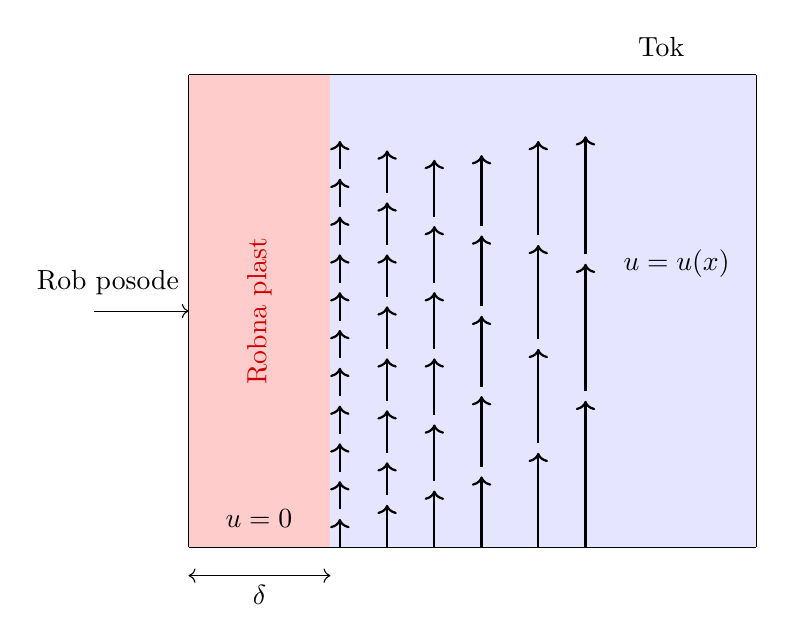
\begin{tikzpicture}[scale=1.2]

  % Draw the container walls
  \draw[thick] (0,0) -- (0,5);
  \draw[thick] (6,0) -- (6,5);
  \draw[thick] (0,5) -- (6,5);
  \draw[thick] (0,0) -- (6,0);

  % Fluid fill (optional blue fill to indicate fluid)
  \fill[blue!10] (0,0) rectangle (6,5);

  % Boundary layer shaded region
  \fill[red!20] (0,0) rectangle (1.5,5);

  % Label the boundary layer
  \node[red!80!black, rotate=90] at (0.75,2.5) {Robna plast};

  % Velocity profile (arrows)
  %\draw[->, thick] (1.5,0.5) -- (5,0.5);
  %\draw[->, thick] (1.5,2.5) -- (5.5,2.5);
  %\draw[->, thick] (1.5,4.5) -- (5,4.5);

  % Velocity labels
  \node[right] at (4.5,3) {$u = u(x)$};
  \node[left] at (1.2,0.3) {$u = 0$};

  % Show arrow and label for Wall (moved to the left)
  \draw[->] (-1, 2.5) -- (0,2.5);
  \node[left] at (0,2.8) {Rob posode};

  % Delta (boundary layer thickness)
  \draw[<->] (1.5,-0.3) -- (0,-0.3);
  \node at (0.75,-0.5) {$\delta$};

  % Free stream label
  \node at (5,5.3) {Tok};

  \draw[->, thick] (1.6,0) -- (1.6,0.3);
  \draw[->, thick] (1.6,0.4) -- (1.6,0.7);
  \draw[->, thick] (1.6,0.8) -- (1.6,1.1);
  \draw[->, thick] (1.6,1.2) -- (1.6,1.5);
  \draw[->, thick] (1.6,1.6) -- (1.6,1.9);
  \draw[->, thick] (1.6,2) -- (1.6,2.3);
  \draw[->, thick] (1.6,2.4) -- (1.6,2.7);
  \draw[->, thick] (1.6,2.8) -- (1.6,3.1);
  \draw[->, thick] (1.6,3.2) -- (1.6,3.5);
  \draw[->, thick] (1.6,3.6) -- (1.6,3.9);
  \draw[->, thick] (1.6,4) -- (1.6,4.3);


  \draw[->, thick] (2.1,0) -- (2.1,0.45);
  \draw[->, thick] (2.1,0.55) -- (2.1,0.9);
  \draw[->, thick] (2.1,1) -- (2.1,1.45);
  \draw[->, thick] (2.1,1.55) -- (2.1,2);
  \draw[->, thick] (2.1,2.1) -- (2.1,2.55);
  \draw[->, thick] (2.1,2.65) -- (2.1,3.1);
  \draw[->, thick] (2.1,3.2) -- (2.1,3.65);
  \draw[->, thick] (2.1,3.75) -- (2.1,4.2);


  \draw[->, thick] (2.6,0) -- (2.6,0.6);
  \draw[->, thick] (2.6,0.7) -- (2.6,1.3);
  \draw[->, thick] (2.6,1.4) -- (2.6,2);
  \draw[->, thick] (2.6,2.1) -- (2.6,2.7);
  \draw[->, thick] (2.6,2.8) -- (2.6,3.4);
  \draw[->, thick] (2.6,3.5) -- (2.6,4.1);
  

  \draw[->, thick] (3.1,0) -- (3.1,0.75);
  \draw[->, thick] (3.1,0.85) -- (3.1,1.6);
  \draw[->, thick] (3.1,1.7) -- (3.1,2.45);
  \draw[->, thick] (3.1,2.55) -- (3.1,3.3);
  \draw[->, thick] (3.1,3.4) -- (3.1,4.15);


  \draw[->, thick] (3.7,0) -- (3.7,1);
  \draw[->, thick] (3.7,1.1) -- (3.7,2.1);
  \draw[->, thick] (3.7,2.2) -- (3.7,3.2);
  \draw[->, thick] (3.7,3.3) -- (3.7,4.3);


  \draw[->, thick] (4.2,0) -- (4.2,1.55);
  \draw[->, thick] (4.2,1.65) -- (4.2,3);
  \draw[->, thick] (4.2,3.1) -- (4.2,4.35);

\end{tikzpicture}
\caption{Posoda, kjer imamo robno plast širine $\delta$ in tokovnice $u$, katerih hitrost se veča, bolk kot smo stran od roba.}
\end{figure}

Ponovno začnemo z Navier-Stokesovo enačbo, vendar predpostavimo, da nimamo vpliva zunanjih
sil tj. $f = 0$.
$$
\frac{\partial u}{\partial t} + (u\cdot \nabla)u = - \frac{1}{\rho}\nabla p + \nu \nabla^2 u.
$$
Enačbo skalarno pomnožimo s hitrostjo $u$
\begin{align*}
u\cdot\frac{\partial u}{\partial t} + (u\cdot \nabla)|u|^2 = - \frac{1}{\rho}(u\cdot\nabla p) + \nu (u\cdot\nabla^2 u)
\end{align*}
Zapišimo vsak člen preko diferencialnega operatorja. Prvi in tretji člen ni težko 
zapisati preko gradienta:
$$
\frac{\partial}{\partial t} \Big(\frac{1}{2} u^2 \Big) = u\cdot \frac{\partial u}{\partial t}.
$$
in
$$
\nabla \cdot (up) = p\underbrace{\nabla\cdot u}_{=0} + u\cdot (\nabla p) = u\cdot (\nabla p)
$$

Za drugi člen, uporabimo pravilo produkta za gradient 
\begin{align*}
\nabla \cdot (|u|^2 u) &= \nabla(|u|^2) \cdot u + |u|^2 \underbrace{(\nabla \cdot u)}_{= 0} =  (2(u\cdot\nabla)u)u\\[2mm]
\Longrightarrow (u\cdot\nabla)|u|^2 &= \nabla \cdot \Big(\frac{1}{2} |u|^2 u\Big).
\end{align*}

Zadnji člen pa lahko zapišemo kot:
$$
u\cdot \nabla^2 u = \nabla\cdot\Big((u\cdot \nabla)u - \nabla\Big(\frac{1}{2} |u|^2\Big)\Big) - |\nabla u|^2,
$$
kjer je 
\begin{equation}
\label{gradnorm}
  |\nabla u|^2 = \sum_{i,j=1}^3 \Big(\frac{\partial u_i}{\partial x_j}\Big)^2.
\end{equation}
Dobljeno enakost 
$$
\frac{\partial}{\partial t} \Big(\frac{1}{2} u^2 \Big) + \nabla \cdot \Big(\frac{1}{2} |u|^2 u\Big) = 
-\frac{1}{\rho}\nabla(p u) + \nu \nabla\cdot\Big((u\cdot \nabla)u - \nabla\Big(\frac{1}{2} |u|^2\Big)\Big) - \nu|\nabla u|^2
$$
integriramo po omejenem območju $\Omega$ z robomo $\partial \Omega$:
\begin{align*}
\int_\Omega \frac{\partial}{\partial t} \Big(\frac{1}{2} u^2 \Big)\dif V + \int_\Omega \nabla \cdot\Big(\frac{1}{2} |u|^2 u
+\frac{1}{\rho}p u - \nu(u\cdot \nabla)u + \nu\nabla\Big(\frac{1}{2} |u|^2\Big)\Big)\dif V =\int_V - \nu|\nabla u|^2 \dif \Omega.\qquad\qquad\qquad
\end{align*}
Po izreku o divergenci:
\begin{align*}
  \int_\Omega \frac{\partial}{\partial t} \Big(\frac{1}{2} u^2 \Big)\dif V + \int_{\partial\Omega} \frac{1}{2} |u|^2 u
  +\frac{1}{\rho}p u - \nu(u\cdot \nabla)u + \nu\nabla\Big(\frac{1}{2} |u|^2\Big)\dif \vec{S} =\int_\Omega - \nu|\nabla u|^2 \dif V.\qquad\qquad\qquad\qquad
\end{align*}
Ker smo prevzeli robni pogoj $u_{|_{\partial\Omega}} = 0$, srednji člen odpade in nam ostane 
$$
\int_\Omega \frac{\partial}{\partial t} \Big(\frac{1}{2} u^2 \Big)\dif V = - \int_\Omega\nu|\nabla u|^2 \dif V
$$
$$
\frac{\partial}{\partial t}\int_\Omega \frac{1}{2} u^2 \dif V = - \nu\int_\Omega |\nabla u|^2 \dif V
$$
\newpage
Kako interpretiramo dani rezultat? Levi stran enakosti nam pove, kako se kinetična energija 
v območju $\Omega$ spreminja s časom. Desni člen je negativen, saj je integrand pozitiven.
Torej kinetična energija toka s časom pada in prehaja v toploto.\\
Lahko pa povemo še malo več. Naj bo $f \neq 0$ in ponovimo postopek. Dobimo identično 
enačbo, le da vsebuje še delo zunanje sile
$$
\frac{\partial}{\partial t}\int_\Omega \frac{1}{2} u^2 \dif V = - \nu\int_\Omega |\nabla u|^2 \dif V + \int_\Omega u\cdot f \dif V.
$$
Če se kinetična energija s časom ne spreminja (miruje) tj. $\frac{\partial}{\partial t} u^2 = 0$:
$$
 \nu\int_\Omega |\nabla u|^2 \dif V = \int_\Omega u\cdot f \dif V.
$$
Ta enakost nam sedaj pove, da je v primeru ko se kinetična energija ohranja, da je 
energija, ki odhaja iz sistema enaka energiji, ki jo dovajamo z delom telesne sile $f$.
Ta rezultat nam da namig, da smo na pravi poti, kar se tiče analize turbulence in tokov
nasplošno, saj je ugotovljeno ekvivalentno 1. zakonu termodinamike:
\begin{definicija}[1. Zakon termodinamike]
Naj bo $\Omega$ sistem oz. omejeno območje. Potem je sprememba energije ($E$) sistema, 
enaka energiji vhodne($E_\text{in}$) in izhodne energije($E_{\text{out}}$)
\begin{equation}
\triangle E = E_\text{in} + E_{\text{out}}.
\end{equation}
\end{definicija}

\begin{definicija}
Naj bo $u$ rešitev Navier-Stokesove enačbe in zadošča zakonu o ohranitvi mase. Potem je 
viskozna disipativnost
\begin{equation}
\epsilon = \nu|\nabla u|^2.
\end{equation}
\end{definicija}

\subsubsection{Velikostne skale}
Ključna ugotovitev v prvi polovici 20. stoletja, ki je spremenila, kako so ljudje gledali 
na turbulenco je, da se kjub njenemu kaotičnemu obnašanju, pojavijo urejene strukture. To 
so vrtinci. V zadnjem razdelku smo videli, da energija pada s časom, na poljubni domeni 
$\Omega$. Jasno je, če je domena večja, bo večji oddok/prenos energije. Če je turbulenten 
tok sestavljen iz vrtincev, se pojavi vprašanje kako veliki oz. majhni so taki vrtinci? 
Ključni so vrtinci "najmanjših" velikosti zaradi naslednjega mehanizma:
energija vrtinca se manjša in se prenaša na manjše vrtince. Ta postopek se ponavlja, dokler 
ne pridemo do vrtincev velikosti, pri katerih se energija ne prenese več na manjše vrtince 
ampak se zaradi viskoznosti energija začne pretvarjati v toploto. Tem vrtincem pravimo
\textbf{disipativni vrtinci}.

Še ena opazka: ko govorimo o velikih vrtincih, govorimo tudi o velikih Reynoldsovih 
številih oz. $Re >> 1$. Spomnimo se, da smo iz brezdimenzijske Navier-Stokesovove enačbe 
dobili Eulerjevo enačbo \ref{Euler NS}, ki ne vsebuje viskoznega člena. To pomeni, da je 
$\nu \nabla^2 u \approx 0$ $\Longrightarrow$ $\epsilon \approx const.$ Zato bomo v 
nadaljevanju predpostavili, da je viskozna disipativnost konstanta (do katerih velikostih 
ima ta predpostavka smisel?).\\

Označimo z $\mathscr{l}$ premer poljubnega vrtnica in z $\mathscr{u}$ povprečna hitrost vrtinca.
Definiramo turbulentno Reynoldsovo število $R_t = \frac{\mathscr{u}\mathscr{l}}{\nu}$. 
V splošnem velja $Re > R_t$, vendar sta primerljiva, zato $R_t >> 1$. \\
Ker smo videli kako pomembna je količina $\epsilon$, jo bomo povezali s količinama 
$\mathscr{l}$ in $\mathscr{u}$ breko dimenzijske analize. Enota za $\frac{\partial u}{\partial x_i}$,
kjer je $i=1,2,3$, je $\frac{m}{s\cdot m} = \frac{1}{s}$, zato je enota za $[|\nabla u|^2] = \frac{1}{s^2}$.
Enota za $\epsilon$ je 
\begin{align*}
[\epsilon] = \nu |\nabla u|^2 = \frac{m^2}{s} \frac{1}{s^2} = \frac{m^2}{s^3}.
\end{align*}
Za primerno izbran čas $\tau$ dobimo oceno
\begin{equation}
\label{hitrost approx}
\epsilon \sim \frac{\mathscr{l}^2}{\tau^3} = \frac{\mathscr{u}^2}{\tau} = \frac{\mathscr{u^3}}{\mathscr{l}},
\end{equation}
kjer je $\mathscr{u} = \frac{\mathscr{l}}{\tau}$.\\
(Paradoks: zakaj je ta izraz neodvisen od $\nu$ medtem ko je definicija odvisna od $\nu$).\\
Se pa izkaže, da to najboljši način za ocenjevati velikosti vrtincev. Velik preskok je 
naredil Andrej Nikolajevič Kolmogorov, ki je postavil hipotezo, da sta hitrost $\upsilon$ 
in dolžina $\eta$ disipativnih vrtincev odvisna le od viskozne disipativnosti $\epsilon$ 
in kinematične viskoznosti $\nu$. Poiščimo izraz zanju.\\
Razdalja $\eta$  se začne, ko začne prevladovati viskozni del Navier-Stokesove enačbe 
$$
\nu \nabla^2 u > (u\cdot \nabla)u.
$$
Aproksimiramo vsakekga posebaj preko brezdimenzijske analize 
\begin{align*}
\nu \nabla^2 u &\sim \nu \frac{\partial^2 u}{\partial x^2} \sim \frac{\nu \mathscr{u}}{\mathscr{l}} = \frac{\nu}{\mathscr{l}\tau}. \\[2mm]
&(u\cdot \nabla)u \sim \frac{\mathscr{u}^2}{\mathscr{l}} \sim \frac{\mathscr{l}}{\tau}
\end{align*}
$$                                                                                                                                                                                                                
\Longrightarrow \nu \nabla^2 u > (u\cdot \nabla)u \iff \frac{\nu}{\mathscr{l}\tau} > \frac{\mathscr{l}}{\tau} \iff \mathscr{l}^2 < \nu \tau.
$$
Iz izraza \ref{hitrost approx} izpostavimo $\tau$, kar nam da:
$$
l^2 < \nu \tau = \nu \Big(\frac{\mathscr{l}^2}{\epsilon} \Big)^\frac{1}{3} \iff l < \Big(\frac{\nu^3}{\epsilon} \Big)^\frac{1}{4}.
$$
Neenakost, nam da območje velikosti vrtincev, ki nimajo za modeliranje velikega pomena. 
Zgornja meja hitrosti teh vrtincev:
\begin{align*}
\upsilon^3 =& \,\mathscr{l}\epsilon = \Big(\frac{\nu^3}{\epsilon}\Big)^\frac{1}{4} \epsilon = (\epsilon \nu)^\frac{3}{4} \\
&\Longrightarrow\, \upsilon = (\epsilon \nu)^\frac{1}{4}.
\end{align*}

\begin{definicija}
Naj bosta $\nu$ viskoznost in $\epsilon$ viskozna disipativnost. Definiramo Kolmogorovovo 
hitrostno skalo 
\begin{equation}
  \upsilon = (\epsilon \nu)^\frac{1}{4}.
\end{equation}
in Kolmogorovo dolžinsko skalo 
\begin{equation}
  \eta = \Big(\frac{\nu^3}{\epsilon} \Big)^\frac{1}{4}.
\end{equation}
To sta  velikost in hitrost najmanjšega možnega vrtinca.
\end{definicija}

Poglejmo si nekaj posledic. Reynoldsovo število disipativnih vrtincev je 
$$
R_t = \frac{\upsilon\eta}{\nu} = (\epsilon \nu)^\frac{1}{4}\,\Big(\frac{\nu^3}{\epsilon} \Big)^\frac{1}{3} \,\frac{1}{\nu} = 1
$$
kar se sklada s z domnevo da ima viskoznost velik vpliv. Poglejmo še koliko večji in 
hitrejši so veliki vrtinci:
\begin{align*}
\frac{\mathscr{l}}{\eta} &= \frac{l \epsilon^\frac{1}{4}}{\nu^\frac{3}{4}} \stackrel{\ref{hitrost approx}}{\sim}
\frac{\mathscr{l} \mathscr{u}^\frac{3}{4}}{\mathscr{l}^\frac{1}{4}\nu^\frac{3}{4}} = \Big(\frac{\mathscr{u}\mathscr{l}}{\nu} \Big)^\frac{3}{4} = R_t^\frac{3}{4}, \\[1mm]
\frac{\mathscr{u}}{\upsilon} &= \frac{u}{(\epsilon \nu)^\frac{1}{4}} \stackrel{\ref{hitrost approx}}{\sim} 
\frac{\mathscr{u}}{\Big(\frac{(\mathscr{l}^3 \eta)}{\mathscr{l}}\Big)^\frac{1}{4}} = 
\Big(\frac{\mathscr{u} \mathscr{l}}{\nu}\Big)^\frac{1}{4} = R_t^\frac{1}{4}.
\end{align*}
Ker je $R_t >> 1$, nam izračun nam pove, da so disipativni vrtinci občutno manjši in 
počasnejši od energijsko bogatih vrtincev. 
\begin{primer}
Tipična hitrost in velikost vrtinca v robni plasti atmosfere sta $\mathscr{u} \sim 1 \frac{m}{s}$ in 
$l \sim 10^3 m$ viskoznost zraka pa je $\nu \sim 10^-5 \frac{kg}{m s}$. Torej je 
$R_t \sim 10^8$, kar nam da oceni za hitrost in velikost disipativnih vrtincev 
$\mathscr{u} \sim 10^{-2} \frac{m}{s}$ in $\eta \sim 10^{-3}m$.
\end{primer}

Z znanjem ki smo ga pridobili do sedaj lahko hitro pokažemo problem modeliranja turbulence
direktno preko Navier-Stokesovih enačb. Ker so najmanjši smiselne dolžine velikosti $\eta$,
velikost območja, ki ga želimo modelirati naj bo $L$. Po zgornjem razmisleku, je število
potrebnih točk 
$$
N = \Big( \frac{L}{\eta} \Big) \sim R_t^\frac{3}{4}
$$
oz. v treh dimenzijah 
$$
N = \Big( \frac{L}{\eta} \Big)^3 \sim R_t^\frac{9}{4}.
$$
Iz zadnjega primera hitro postane jasno, da je modeliranje direktno preko danih enačb 
povsem nepraktično, saj je število potrebnih točk približno $N \sim (10^8)^\frac{9}{4}
= 10^{18}$. Zato so direktne numerične simulacije uporabljajo le za manjša območja, 
naprimer $R_t \sim 1000$, torej $N \sim 10^\frac{27}{4} \sim 10^7$, kar še vedno ni 
majhna številka. 

\newpage
\section{Large eddy simulacije}

Nakoncu zadnjega poglavja smo videli, da je direktno reševanje Navier-Stokesovih enačb 
za velike vrtince oz. tri dimenzijonalno turbulentno gibanje tokov. V tem poglavju 
bomo spoznali orodja s katerimi bomo enačbe, ki opisujejo dane tokove, priredili na tak
način, da bomo lahko bolj učinkovito rešili enačba. Simulacije velikih vrtincev (eng. 
Large eddy simulations) oz. LES razdelimo na štiri korake 
\begin{enumerate}
\item[i)] Spoznali bomo kocept povprečenja in kako tok razcepimo na dva dela: 
povprečni del in spremenljivi del. Povprečni del bo predstavljal hitrostno polje 
velikih vrtincev. Osredotočili se bomo na posebno vrsto povprečja, to je filtracija.
\item[ii)] Preko filtracije Navier-Stokesovih enačb dobimo nove enačbe, ki jih bomo 
uporabili za numerično reševanje. 
\item[iii)] Zaprtje novih enačb. Pri prejšnji točki dobimo nove člene v enačbi, kar 
povzroči, da imamo več spremenljivk kot enačb. Problem bomo rešili z modeliranjem 
novih členov.
\item[iv)] Numerično rešimo zaprt sistem enačb, ki opisuje tok.
\end{enumerate}

To je najbolj splošen pristop, je pa pomembno navesti, da obstaja več podvrst LES, 
ki so odvisne od kompleksnosti in velikosti območja, ki ga obravnavamo.

\subsection{Povprečja}

Vse odvisne spremenljivke, hitrost, vrtinčnost, tlak, temperatura \dots, so turbulentne.
Intuitivno to pomeni, da so v prostori neenakomerno porazdeljene in v vsaki točki v 
opazovanem območju kaotično oscilirajo. Zaradi naključnega obnašanja je pogosto smiselno turbulenco 
analizirati z vidika statiske. V delu se temu ne bomo posvetili, omenimo zaradi 
povprečja, ki temelji na več ponovitvah istega poskusa. \\
Ideja za povprečji je, da hitrostno polje $U(x, t)$ razcepimo na povprečni del $\overline{U}(x, t)$ in 
oscilirajoči del $u(x, t)$.
\begin{equation}
U(x, t) = \overline{U}(x,t) + u(x, t).
\end{equation}
Temu razcepu pravimo Reynoldsov razcep.

Zapišimo nekaj lastnosti, ki jih želimo od povprečji. Naj bosta $U$ in $V$ dva tokova in 
$\alpha, \beta \in \R$:
\begin{enumerate}
  \item[i)] Linearnost: 
  $$\overline{\alpha U + \beta V} = \alpha \overline{U} + \beta\overline{V}.$$
  \item[ii)] Povprečje konstante $C$ je $C$:
  $$ \overline{C} = C.$$
  \item[iii)] Indempotentnost:
  $$ \overline{\overline{U}} = \overline{U}.$$
  \item[iv)] Povprečje oscilirajočega dela je $0$:
  $$ \overline{u} = \overline{U - \overline{U}} = 0.$$
  \item[v)] Pravilo produkta: 
  $$ \overline{U\cdot V} = \overline{U}\cdot \overline{V}. $$
  \item[vi)] Komutiranje z odvajanjem:
  $$ \overline{\frac{\partial U}{\partial x_i}} = \frac{\partial \overline{U}}{\partial x_i}.$$
\end{enumerate}

\begin{lema}
Če velja lastnost $i)$ potem je $iii) \iff iv)$
\end{lema}

\begin{proof}
\begin{align*}
\overline{\overline{U}} = \overline{U} \iff 0 = \overline{U} - \overline{\overline{U}} \stackrel{i)}{=} 
\overline{U - \overline{U}}.
\end{align*}
\end{proof}


\subsubsection{Ansambelsko povprečje}
Recimo, da opravljamo eksperiment in dobimo nek rezultat. Pogostokrat zaradi napak ali 
zunanjih vplivov ali majhne verjetnosti pojava željenega rezultata poskus večkrat ponovimo in 
za naš končni rezultat vzamemo povprečje vseh rezultatov. To je ideja za ansambelskim 
povprečenjem.

Pri tokovih turbulenca predstavlja naša odstopanja ali šum oz. kaotičen del.
Ker se pri zelo majhnih začetnih pogojih, tok lahko zelo spremeni, nam vsaka ponovitev 
poskusa, da novo rešitev, lahko zgleda zelo drugačna od prejšne in naslednje. 
Tem ponovitvam pravimo realizacije in označimo $U(x, t; \alpha)$, za $\alpha \in \N$
realizacijsko število. 
\begin{definicija}
Ansambelsko povprečje toka $U$ je 
\begin{equation}
U^\text{avg}(x, t) = \lim_{N\rightarrow \infty} \frac{1}{N}\sum_{\alpha=1}^N U(x, t;\alpha). 
\end{equation}
\end{definicija}

Bolj formalno, na $U(x, t;\alpha)$ gledamo kot slučajni vektor, in zaporedje 
$U(x, t; 1)$, $U(x, t; 2)$ \dots, $U(x, t;n)$ je zaporedje neodvisno, enako porazdeljenih 
slučajnih vektorjev. Pričakovana vrednost $E(U_i) = \mu$ za vsak $i\in\N$, zato je po 
zakonu velikih števil Ansambelsko povprečje konvergentno.\\

Ansambelsko povprečje zadošča vsem lastnostim $i) - vi)$ zato je temelj za \\
Reynoldsovo-povprečene Navier-Stokesove simulacije (RANS). Omenimo še dve povprečji: 
\begin{definicija}
Časovno povprečje je 
\begin{equation}
U^T(x, t; T) = \frac{1}{T}\int_0^T U(x, t + \tau) \dif \tau.
\end{equation}
\end{definicija}

\begin{definicija}
Prostorsko povprečje je 
\begin{equation}
U^T(x, t; L) = \frac{1}{L}\int_0^L U(x + s, t) \dif s.
\end{equation}
\end{definicija}

Čeprav so ta povprečja na prvi pogleda nepovazana, pa se v praksi izkaže, da imajo poseben 
pomen. Naj bo polje $U$ stacionarno tj. $U(x, t) = U(x)$ ali homogeno oz. $U(x, t) = U(t)$.
Intuitivno bi pričakovali, da je 
$$
\lim_{T\rightarrow \infty} U^T(x, t; T) = \lim_{T\rightarrow \infty} U^T(x; T) = U^\text{avg}(x)
$$
oz. 
$$
\lim_{T\rightarrow \infty} U^S(x, t; S) = \lim_{T\rightarrow \infty} U^S(t; T) = U^\text{avg}(t)
$$
Če slučajna spremenljivka $U $oz. hitrostno polje v našem primeru, zadošča obema lastnostima, 
pravimo, da je $U$ \textbf{ergodično}. V računski dinamiki fluidov se pogosto predpostavi, da je turbulenca ergodična. 
Temu pravimo ergodična hipoteza. Zato ne obstaja dokaz, vendar mnoge numerične simulacije potrjujejo hipotezo 
in eksperimenti hipotezo potrjujejo. \\
Ergodičnost se predpostavi, saj je računanje ansambelskega povprečja težavno, ker potrebujemo 
veliko poskusov za njegov izračun, med tem ko je prostorko ali časovno povprečje dokaj 
enostavno.

\subsubsection{Filtracija}

Sedaj se bomo resno posvetili filtraciji, ki je posebna vrsta povprečja.
\begin{definicija}
Naj bo $U: \R^d\times \R^+ \rightarrow \R^3$ vektorsko polje in $G: \R^d\times \R^d \rightarrow \R$.
Potem je filter polja $U$, polje filtrirano polje $\overline{U}$
\begin{equation}
\overline{U}(x, t) = \int_{\R^d} G(r, x)U(x-r, t) \dif r.
\end{equation}
Funkciji $G$ pravimo filtracijska funkcija in zadošča normalizacijskem pogoju 
$$
\int_{\R^d} G(r, x) \dif r = 1.
$$
\end{definicija}

\begin{definicija}
Naj bo $G$ filtracijska funkcija in $U$ tok. Potem je residualno polje 
\begin{equation}
u'(x, t) = U(x, t) - \overline{U(x, t)}.
\end{equation}
\end{definicija}

\begin{opomba}
  \hfill
\begin{itemize}
\item Polji $\overline{U}$ in $u$ bomo tudi imenovali razrešen del in podfilterska skala.
\item Opazimo, da je definicija filtra skoraj identična definiciji konvolucije, le da je  
$U$ vektorsko polje in ne skalar, kot običajno.
\item Zgornji razcep je analogen Reynoldsovem razcepu, glavna razlika je, da rezidualni 
del ni nujno enak $0$
$$ \overline{u'} \neq 0.$$
\end{itemize}
\end{opomba}

\begin{trditev}
Filtracija zadošča lasnostim $i), ii)$ in kumutarnju z časovnim odvodom. Če je filtracijska funkcija $G$ homogeno, velja lasnost $vi)$.
\end{trditev}

\begin{proof}
\begin{enumerate}
  \item[i)] Naj bosta $U$, $V$ vektorski polji, $\alpha, \beta \in \R$ in $G$ filtracijska 
  funkcija
  \begin{align*}
  \overline{\alpha U + \beta V} &= \int_{\R^d} G(r, x) (\alpha U(x-r, t) + \beta V(x-r, t)) \dif r = \\
  &= \int_{\R^d} \alpha G(r, x) U(x-r, t) + \beta G(r, x) V(x-r, t) \dif r = \\
  &= \alpha\int_{\R^d} G(r, x) U(x-r, t)\dif r + \beta\int_{\R^d}G(r, x) V(x-r, t) \dif r = \\
  &= \alpha \overline{U} + \beta\overline{V}
  \end{align*}
  \item[ii)] Naj bo $C\in \R^3$ in $G$ filtracijska funkcija
  \begin{align*}
  \overline{C} = \int_{\R^d} G(r, x) C \dif r = \Big(\underbrace{\int_{\R^d} G(r, x)\dif r}_{\substack{\text{normalizacijski}\\\text{pogoj}}}\Big) C = C.
  \end{align*}
  \item[vi)] Naj bo $U$ odvedljivo vektorsko polje po časovni spremenljivki in $G$ filtracijska funkcija 
  \begin{align*}
  \frac{\dif}{\dif t} \overline{U}(x, t) &= \frac{\dif}{\dif t} \int_{\R^d} G(r, x) U(x-r, t) \dif r = \\
  &= \mathcal{F}^{-1}\mathcal{F}\Big(\frac{\dif}{\dif t} \int_{\R^d} G(r, x) U(x-r, t) \dif r\Big)= \\
  &= \mathcal{F}^{-1}\Big(i\omega \mathcal{F}\Big(\int_{\R^d} G(r, x) U(x-r, t) \dif r \Big)\Big)= \\
  &= \mathcal{F}^{-1}(i\omega \hat{G}(\omega, x)\hat{U}(x, \omega)) = \\
  &= \mathcal{F}^{-1}(\hat{G}(\omega, x) \cdot(i\omega \hat{U}(x, \omega))) = \\
  &= \int_{\R^d} G(r, x) \frac{\dif}{\dif t} U(x-r, t) \dif r =\\[1mm]
  &= \overline{\frac{\dif U}{\dif t}}.
  \end{align*}

  Odvajamo še po času in predpostavimo, da lahko zamenjamo vrstni red odvajanja in integracije 
  (kateri pogoji so smiselni, da je to izpolnjejo ali si isti kot pri zgornjem izračunu?) 
  \begin{align*}
  \frac{\!\!\dif}{\dif x_i} \overline{U}(x, t) &= \frac{\dif}{\dif x_i} \int_{\R^d} G(r, x) U(x-r, t) \dif r = \\
  &=  \int_{\R^d} \frac{\dif}{\dif x_i} (G(r, x) U(x-r, t)) \dif r = \\
  &=  \int_{\R^d} \frac{\dif G}{\dif x_i}(r, x)  U(x-r, t) \dif r + \int_{\R^d} G(r, x)  \frac{\dif U}{\dif x_i}(x-r, t) \dif r = \\
  &= \int_{\R^d} \frac{\dif G}{\dif x_i}(r, x)  U(x-r, t) \dif r + \overline{\frac{\dif U}{\dif x_i}}.
  \end{align*}

  $G$ je homogena torej je $G(r, x) = G(r)$, posledično 
  $$\frac{\dif G}{\dif x_i}(r, x) = \frac{\dif G}{\dif x_i}(r) = 0$$
  in enakost sledi.
\end{enumerate}
\end{proof}

\begin{opomba}
  \hfill
\begin{itemize}
  \item Ker je $U$ vektor, integral deluje po komponentah, zato tudi Fourierova tranformacija deluje po komponentah. 
  \item V dokazu smo uporabili dejstvo 
  $$ \mathcal{F}(f')(\omega) =  i\omega \mathcal{F}(f)(\omega). $$
\end{itemize}
\end{opomba}

\noindent
Poglejmo si dva filtra, ki se pogosto uporabljata. Primera si bomo pogledali v eni dimenziji, 
kar se enostavno  posploši v višje dimenzije. Od sedaj naprej bomo predpostavili, da je 
$G$ homogeno tj. $G(r, x) = G(r)$. Matematično, je filter sedaj konvolucija, kar običajno 
zapišemo
\begin{equation}
\overline{U}(x, t) = (U * G)(x, t).
\end{equation}
Iz konvolucijskega izreka dobimo 
\begin{equation}
\hat{\overline{U}} = \mathcal{F}(\overline{U})(\xi, t) = \mathcal{F}(U)(\xi, t)\cdot \mathcal{F}(G)(\xi)= 
\hat{U}(\xi, t)\cdot \hat{G}(\xi).
\end{equation}
\\[1mm] 

\noindent
\textbf{Valovni preklopni filter:} \\
Pokazali smo, da filter zadošča lastnostim $i), ii)$ in $vi)$. Ali lahko za pravo izbiro 
$G$ dodatno zadostimo še kateri od ostalih lastnosti? Zaradi linearnosti filtra, nam 
ostaneta le dve lastnosti: Indempotentnost in pravilo produkta. Pravilo produkta bo
zadoščeno, če bo za pravo funkcijo $G$, integral multiplikativen. Take funkcije sicer 
obstajajo, vedar so zelo raznolike in običajno nimajo fizikalnega pomena. Torej nam ostane 
le indempotentnost. Poglejmo, kako se izraža $\overline{\overline{U}}$ preko konvolucije:
\begin{align*}
\overline{\overline{U}}(x, t) &= \int_{\R} G(r) \overline{U}(x - r, t) \dif r = \\
&= \int_{\R} G(r) \int_{\R} G(s) U(x-r-s, t) \dif s \dif r = \\
&= \int_{\R} (G*U)(x - r, t) \dif r = G*(G * U)(x, t) \\[1mm]
&\Longrightarrow \mathcal{F}(\overline{\overline{U}})(\xi, t) = \mathcal{F}(G)^2(\xi)\cdot\mathcal{F}(U)(\xi, t) = \hat{G}^2(\xi) \cdot \hat{U}(\xi, t)
\end{align*}
Če želimo, da je $G$ indempotent
\begin{align*}
\overline{U} &= \overline{\overline{U}} \\
\hat{U}\hat{G} &= \hat{U}\hat{G}^2 \\ 
(\hat{G}^2 - &\hat{G}) = 0.
\end{align*}
To pomeni, da lahko $G$ zavzame le vrednosti $0$ in $1$. Preden si poglemo bolj specifičen primer, 
si poglejmo problem preko Fourierove vrste, kar bo pomembno pri analizi v nadaljevanju.
$U$ razvijemo v kompleksno Fourierovo vrsto na intervalu $[0, L]$ za $L > 0$
\begin{equation}
U(x, t) = \sum_{n=-\infty}^\infty a_n(t) e^{i\kappa_n x},
\end{equation}
kjer je $\kappa_n = 2\pi\frac{n}{L}$. Filtriramo ta razvoj 
\begin{align*}
\overline{U}(x, t) &= \int_{\R^d} G(r) U(x - r, t) \dif r = \\
&= \int_{\R^d} G(r) \sum_{n=-\infty}^\infty a_n(t) e^{i\kappa_n (x - r)} \dif r = \\
&= \sum_{n=-\infty}^\infty a_n(t)\Big(\int_{\R^d} G(r) e^{-i\kappa_n r}\Big) e^{i\kappa_n x}\dif r = \\
&= \sum_{n=-\infty}^\infty a_n(t) \hat{G}(\kappa_n) e^{i\kappa_n x},
\end{align*}
Kot prej je $\hat{G}$ Fourierova transformiranka funkcije $G$ 
$$
\hat{G}(\kappa) = \int_{\R^d} G(r) e^{-i\kappa r} \dif r
$$
in preko inverzne Fourierove tranformacije dobimo
$$
G(x) = \frac{1}{2\pi} \int_{\R^d} \hat{G}(\kappa) e^{i\kappa x} \dif \kappa.
$$
\begin{opomba}
V literaturi se $\hat{G}$ pogosto imenuje prenosna funkcija in se označi s $T$.
\end{opomba}

\noindent
Uporabimo filter na $\overline{U}$
\begin{align*}
\overline{\overline{U}}(x, t) &= \int_\R G(r) \overline{U}(x-r, t) \dif r = \\
&= \int_\R G(r) \sum_{n=-\infty}^\infty a_n(t) T(\kappa_n) e^{i\kappa_n (x - r)} \dif r= \\
&= \sum_{n=-\infty}^\infty a_n(t)T(\kappa_n) e^{i\kappa_n x} \int_\R G(r)e^{-i\kappa_n r} \dif r = \\
&= \sum_{n=-\infty}^\infty a_n(t)T^2(\kappa_n) e^{i\kappa_n x} \dif r
\end{align*}
Primerjamo koeficiente vrst
$$
T^2(\kappa_n) = T(\kappa_n), \quad n\in \Z
$$
kar se ujema z dosedaj ugotovljenim. Ta je izpeljava pomembna ker uvede količino 
$\kappa_n$, ki jo imenujemo $n$-to valovno število. To bo ključno za razreševanje 
polja $\overline{U}$ na diskretni množici (kar je potrebno za numerično modeliranje).
Definiramo nizko-prehodno prenosno funkcijo
$$
T_c(\kappa)=\left\{\begin{array}{l}
  1 ;\,\, |\kappa| \leq \kappa_c \\
  0 ;\,\, |\kappa| > \kappa_c
\end{array}\right.
$$
$\kappa_c \in \R$ se imenuje \textbf{preklopno valovno število}. Sedaj lahko izračunamo 
filtracijsko funkcijo $G$
\begin{align*}
G(x) &= \frac{1}{2\pi} \int_\R T_c(\kappa) e^{-i\kappa x} \dif \kappa = \\
&= \frac{1}{2\pi} \int_{-\kappa_c}^{\kappa_c} e^{-i\kappa x} \dif \kappa = \\ 
&= \frac{i}{2\pi x} e^{-i\kappa x}\Big|_{-\kappa_c}^{\kappa_c} = \\
&= \frac{i}{2\pi x} (e^{-i\kappa_c x} - e^{i\kappa_c x}) = \frac{\sin(\kappa_c x)}{\pi x}.
\end{align*} 

\begin{definicija}
Enodimenzionalni valovno preklopni filter je filter s filtracijsko funkcijo $G$
\begin{equation}
G(x) = \frac{\sin(\kappa_c x)}{\pi x}.
\end{equation}
\end{definicija}
\noindent
To lahko enostavno posplošimo na poljubno dimenzijo 
\begin{definicija}
Za $n\in \N$ definiramo $n$-dimenzionalni valovno preklopno filtracijsko 
funkcijo $G_n$
\begin{equation}
G_n(x) = \prod_{i=1}^n G(x_i) =\prod_{i=1}^n \frac{\sin(\kappa_c x_i)}{\pi x_i}.
\end{equation} 
\end{definicija}


\begin{opomba}
Lahko tudi definiramo visoko-prehodno prenosno funkcijo
$$
T_c(\kappa)=\left\{\begin{array}{l}
  1 ;\,\, |\kappa| \geq \kappa_c \\
  0 ;\,\, |\kappa| < \kappa_c,
\end{array}\right.
$$
vendar v tem filtracijska funkcija ne obstaja.
\end{opomba}


\noindent
\textbf{Škatlast filter:}\\
Nekoliko bolj naravna filtracijska funkcija, ki nas spomne prostorsko povprečje je 
škatlasta funkcija 
\begin{definicija}
Naj bodo $\Delta > 0$. Škatlasta funkcija je 
\begin{equation}
G(x)= \begin{cases}\frac{1}{\Delta} & ; x \in\left[-\frac{\Delta}{2}, \frac{\Delta}{2}\right] \\ 0 & ; \text { sicer }\end{cases}
\end{equation}
\end{definicija}

Prenosno funkcijo lahko izračunamo po zgoraj izpeljani formuli, kar nam da 
$$
T(\kappa) = \frac{\sin(\kappa \frac{\Delta}{2})}{\kappa \frac{\Delta}{2}}.
$$
Navedimo še večdimenzionalno škatlasto funkcijo
\begin{definicija}
Naj bodo $\Delta_1, \dots, \Delta_n > 0$. $n$-dimenzionalna
škatlasta funkcija je 
\begin{equation}
  G(x_1, \dots, x_n)= \begin{cases}\frac{1}{\prod_{i=1}^{n}\Delta_i} & ; x_i \in\left[-\frac{\Delta_i}{2}, \frac{\Delta_i}{2}\right] \\ 0 & ; \text { sicer }\end{cases}
\end{equation}  
\end{definicija}

\begin{opomba}
  \hfill
  \begin{itemize}
    \item Temu filtri se tudi pravi lokalno povprečje.
    \item V literaturi se občasno pojavi tudi nekoliko drugačna definicija. kjer 
    se integrira po krogli namesto po kvadratu.
  \end{itemize}
  \end{opomba}
  

\noindent
\textbf{Gaussov filter}:
Poglejmo filtracijsko funkcijo, ki se razlikuje od prejšnij dveh primerov v dveh pogledih.
Za filtracijsko funkcijo vzamemo Gaussovo funkcijo, ki za razliko od prejšnji dveh 
primeov zvezna in pomembneje pozitivna
\begin{definicija}
Naj bo $\sigma > 0$. Gaussov filter je filter dan z Gaussovo funkcijo 
\begin{equation}
G(x_1, \dots, x_n) = \frac{1}{\sqrt{2\pi}\sigma} e^{-\frac{x^2}{2\sigma^2}}.
\end{equation}
oz. $n$-dimenzionalni Gaussov filter je dan z 
\begin{equation}
G(x_1, \dots, x_n) = \frac{1}{(2\pi \sigma^2)^{n/2}} e^{-\frac{1}{2\sigma^2}(x_1^2 + \dots + x_n^2)}
\end{equation}
\end{definicija}


\subsection{Filtrirani ohranitveni zakoni}

Sedaj je čas, da uporabimo filter na enačbah, ki jih želimo numerično rešiti. V 
razdelku bomo predpostavili, da je filtracijska funkcija homogena, saj bomo potrebovali 
lastnost komutiranja filtra z odvajanjem. Do nadaljnega bomo dodatno predpostavili, 
da je $G$ poljubna, kasneje ko se bomo posvetili natančnejši analizi, jo bomo specificirali.

\subsubsection{Filtriran zakon o ohranitvi mase}

Zakon:
$$
\nabla\cdot U = \sum_{i=1}^3 \frac{\partial U}{\partial x_i} = 0.
$$
\noindent
Filtrirana enačba 
\begin{align*}
\overline{\nabla\cdot U}= \overline{\sum_{i=1}^3 \frac{\partial U}{\partial x_i}} = 
\sum_{i=1}^3 \frac{\partial \overline{U}}{\partial x_i} = \nabla\cdot \overline{U} = 0.
\end{align*}
\noindent
Filtriran zakon:
\begin{equation}
\nabla\cdot\overline{U} = 0.
\end{equation}

\subsubsection{Filtriran zakon o ohranitvi gibalne količine}

Zakon: 
$$
\frac{\partial U}{\partial t} + (U\cdot \nabla)U = -\frac{1}{\rho} \nabla U + \nu\nabla^2 U + f.
$$

\noindent
Preden enačbo filtriramo, jo bomo preoblikovali, da se znebimo nelinearnega člena ($U\cdot \nabla)U$.
Najprej ga razpišemo, po komponentah 
\renewcommand{\arraystretch}{2.5} % default is 1
\[
(U \cdot \nabla) U =
\begin{pmatrix}
U_1 \dfrac{\partial U_1}{\partial x_1} + U_2 \dfrac{\partial U_1}{\partial x_2} + U_3 \dfrac{\partial U_1}{\partial x_3} \\
U_1 \dfrac{\partial U_2}{\partial x_1} + U_2 \dfrac{\partial U_2}{\partial x_2} + U_3 \dfrac{\partial U_2}{\partial x_3} \\
U_1 \dfrac{\partial U_3}{\partial x_1} + U_2 \dfrac{\partial U_3}{\partial x_2} + U_3 \dfrac{\partial U_3}{\partial x_3}
\end{pmatrix} = \Big[\sum_{k=1}^3 U_k \frac{\partial U_j}{\partial x_k}\Big]_j
\]
in pogledamo kako se odvod produkta izraža 
$$
\sum_{k=1}^3 \frac{\partial}{\partial x_k} (U_k U_j) = \sum_{k=1}^3 \Big(U_k\frac{\partial U_j}{\partial x_k}
+ U_j\frac{\partial U_k}{\partial x_k}\Big) = (U\cdot \nabla)U + (\underbrace{\nabla\cdot U}_{\substack{\text{ohranitev}\\{\text{mase}}\\=0}}) U
= (U\cdot \nabla)U.
$$
Levo stran enakosti lahko bolj kompaktno zapišemo
$$
\sum_{k=1}^3 \frac{\partial}{\partial x_k} (U_k U_j) = \nabla \cdot (U_j U) = 
\nabla \cdot [U U^T]_{j} = \nabla \odot [U U^T],
$$

kjer je $U\times U$ Hadamardov produkt oz. produkt po komponentah 
\[
A \odot B = \left[ a_j \cdot b_j \right]_j.
\]
Ta zapis ni najbolj praktičen, zato bomo Navier-Stokesovo enačbo filtrerali po komponentah.
Za $j\in \{1, 2, 3\}$ imamo 
\begin{align*}
\frac{\partial U_j}{\partial t} + \nabla\cdot(U_j U) = -\frac{1}{\rho} \frac{\partial p}{\partial x_j} + \nu\nabla^2 U_j + f_j.
\end{align*}

Filtriramo enačbo, kjer upoštevamo, da filtracija komutira z odvajanjem:
\begin{align*}
  \frac{\partial \overline{U}_j}{\partial t} + \nabla\cdot(\overline{U_j U}) = -\frac{1}{\rho} \frac{\partial \overline{p}}{\partial x_j} + \nu\nabla^2 \overline{U}_j + \overline{f}_j.
\end{align*}
Enačbo lahko zapišemo še bolj kompaktno, če uporabimo Einsteinovo konvencijo 
$$
\sum_{i=1}^n a_i b_i = a_i b_i.
$$
Filtriran zakon:
\begin{equation}
\frac{\partial \overline{U}_j}{\partial t} + \frac{\partial \overline{U_i U_j}}{\partial x_i} = -\frac{1}{\rho} \frac{\partial \overline{p}}{\partial x_j} + \nu \frac{\partial^2 \overline{U}_j}{\partial x_i \partial x_i} + \overline{f}_j.
\end{equation}

\subsubsection{Filtriran zakon o ohranitvi vrtinčnosti}

Zakon:
$$
\frac{\partial \omega}{\partial t} + (U\cdot \nabla)\omega = (\omega \cdot \nabla)U + \nu \nabla^2 \omega + \nabla \times f. 
$$
Podobno kot pri Navier-Stokesovih enačbah, bomo prepisali nelinearna člena v bolj primerno 
obliko
\begin{align*}
(U \cdot \nabla) \omega = \Big[\sum_{k=1}^3 U_k \frac{\partial \omega_j}{\partial x_k}\Big]_j\\
(\omega \cdot \nabla) U= \Big[\sum_{k=1}^3 \omega_k \frac{\partial U_j}{\partial x_k}\Big]_j.
\end{align*}
Fiksiramo komponento $j\in\{1, 2, 3\}$ in pogledamo odvod produkta komponent vrtinčnosti in hitrostnega polja:
\begin{align*}
\frac{\partial}{\partial x_i} (U_i \cdot\omega_j) = \sum_{i=1}^3 \frac{\partial}{\partial x_i} (U_i \cdot\omega_j) = 
\sum_{i=1}^3 \omega_j\frac{\partial U_i}{\partial x_i} + U_i\frac{\partial \omega_j}{\partial x_i} = 
\omega_j (\underbrace{\nabla \cdot U}_{\substack{\text{ohranitev}\\\text{mase}\\=0}}) + (U\cdot\nabla)\omega
\end{align*}
\begin{align*}
\frac{\partial}{\partial x_i} (\omega_i \cdot U_j) = \sum_{i=1}^3 \frac{\partial}{\partial x_i} (\omega_i \cdot U_j) = 
\sum_{i=1}^3 U_j\frac{\partial \omega_i}{\partial x_i} + \omega_i\frac{\partial U_j}{\partial x_i} = 
U_j (\underbrace{\nabla \cdot \omega}_{\substack{\text{divergenca}\\\text{rotorja}\\=0}}) + (\omega\cdot\nabla)U.
\end{align*}
Zakon zapisan v komponetnem zapisu je, pri $j\in \{1, 2, 3\}$:
\begin{equation}
\frac{\partial \omega_j}{\partial t} + \frac{\partial}{\partial x_i} (U_i \cdot \omega_j) = 
\frac{\partial}{\partial x_i} (\omega_i \cdot U_j) + \nu \nabla^2 \omega_j + \tilde{f_j}
\end{equation}
za $\tilde{f}_j = [\nabla \cdot f]_j$.\\
Filtriran zakon:
\begin{equation}
  \frac{\partial \overline{\omega_j}}{\partial t} + \frac{\partial}{\partial x_i} \overline{U_i \cdot \omega_j} = 
  \frac{\partial}{\partial x_i} \overline{\omega_i \cdot U_j} + \nu \nabla^2 \overline{\omega_j} + \overline{\tilde{f_j}}.
\end{equation}

\subsubsection{Filtriran zakon o ohranitvi skalarja}

Zakon:
$$
\frac{\partial c}{\partial t} + U\cdot\nabla c = \gamma \nabla^2 c.
$$
V tem primeru bo filtracija enostavna, saj lahko zaradi ohranitva mase, polje $U$ 
potegnemo znotraj gradienta in upoštevamo linearnos filtracije. \\
Filtriran zakon:
\begin{equation}
\frac{\partial \overline{c}}{\partial t} + \nabla \cdot (\overline{cU}) = \gamma \nabla^2 \overline{c}.
\end{equation}

\subsubsection{Filtriran materialni odvod}

Izpeljane enačbe smo sicer prevedli na enačbe primernejše za modeliranje (pomen filtra bomo 
pokazali v naslednjem razdelku), vendar če, na primer, primerjamo filtrirano in 
ne filtrirano Navier-Stokesovo enačbo, sta enačbi fundementalno drugačni, saj imamo 
v drugem členu v enem primeru odvod skalarja $\overline{U_i U_j}$ v drugem pa odvod produkta 
skalarjev $U_i U_j$. Radi bi torej v filtrirani enačbi uvedli člen $\overline{U_i} \cdot \overline{U_j}$.
Vendar pa se pojavi problem, saj $\overline{U_i}\overline{U_j} - \overline{U_i U_j}$. 
\begin{definicija}
Naj bo $U$ vektorsko polje in $\overline{U}$ njena filtracija. Količini 
\begin{equation}
\tau_{ij}^R = \overline{U_i U_j} - \overline{U_i} \,\overline{U_j}
\end{equation}
pravimo \textbf{rezidualni napetostni tenzor}.
\end{definicija}

Iz definicije tenzorja $\tau^R$ se naravno pojavita dodatni definiciji
\begin{definicija}
Rezidualna kinetična energija je 
\begin{equation}
k_r = \frac{1}{2} \tau_{ii}^R = \frac{1}{2}\text{tr}(\tau^R).
\end{equation}
\end{definicija}

\begin{definicija}
\textbf{Izotropni rezidualni napetostni tenzor} je dan z 
\begin{equation}
\tau_{ij}^\text{izo} = \frac{2}{3} k_r \delta_{ij}
\end{equation}
\textbf{anizotropni rezidualni napetostni tenzor} pa z 
\begin{equation}
\tau_{ij}^\text{anizo} = \tau_{ij}^R - \tau_{ij}^\text{izo}.
\end{equation}
\end{definicija}

Zapišemo filtrirano Navier-Stokesovo enačbo preko teh definicij
\begin{align*}
\frac{\partial \overline{U}_j}{\partial t} + &\frac{\partial \overline{U_i U_j}}{\partial x_i} = 
\frac{\partial \overline{U}_j}{\partial t} + \frac{\partial}{\partial x_i} (\overline{U_i}\, \overline{U_j} + \tau_{ij}^R) = 
\frac{\partial \overline{U}_j}{\partial t} + \frac{\partial}{\partial x_i} \overline{U_i}\, \overline{U_j} + \frac{\partial}{\partial x_i} \tau_{ij}^R\\[2mm]
&\Longrightarrow \,\,
\frac{\partial \overline{U}_j}{\partial t} + \frac{\partial \overline{U_i}\, \overline{U_j}}{\partial x_i} = -\frac{1}{\rho} \frac{\partial \overline{p}}{\partial x_j} 
- \frac{\partial \tau_{ij}^R}{\partial x_i}+ \nu \frac{\partial^2 \overline{U}_j}{\partial x_i \partial x_i} + \overline{f}_j.
\end{align*}

Zapišemo še preko $\tau^\text{anizo}$ tenzorja:
\begin{align*}
&-\frac{1}{\rho} \frac{\partial \overline{p}}{\partial x_j} - \frac{\partial \tau_{ij}^R}{\partial x_i}+ \nu \frac{\partial^2 \overline{U}_j}{\partial x_i \partial x_i} + \overline{f}_j = \\[1mm]
&-\frac{1}{\rho} \frac{\partial \overline{p}}{\partial x_j} - \frac{\partial (\tau^\text{izo} + \tau^\text{anizo}) }{\partial x_i}+ \nu \frac{\partial^2 \overline{U}_j}{\partial x_i \partial x_i} + \overline{f}_j = \\[1mm]
&-\frac{1}{\rho} \frac{\partial (\overline{p} + \rho\tau^\text{izo})}{\partial x_j} - \frac{\partial \tau^\text{anizo} }{\partial x_i}+ \nu \frac{\partial^2 \overline{U}_j}{\partial x_i \partial x_i} + \overline{f}_j \\[2mm]
&\Longrightarrow 
\frac{\partial \overline{U}_j}{\partial t} + \frac{\partial \overline{U_i}\, \overline{U_j}}{\partial x_i} = -\frac{1}{\rho} \frac{\partial \overline{P}}{\partial x_j} 
- \frac{\partial \tau_{ij}^\text{anizo}}{\partial x_i}+ \nu \frac{\partial^2 \overline{U}_j}{\partial x_i \partial x_i} + \overline{f}_j,
\end{align*}
kjer je $\overline{P} = \overline{p} + \rho\tau^\text{izo}$ modiciran filtriran tlak 
(zakaj se ga uvede?). Iz te enačbe je jasno kako definirati filtrirani materialni odvod 
\begin{definicija}
Filtriran materialni odvod za vektorko polje $U$ je 
\begin{equation}
\frac{\overline{D}}{\overline{D}t} = \frac{\partial}{\partial t} + \overline{U}\cdot \nabla.
\end{equation}
\end{definicija}

\subsection{Razreševanje filtriranih polj}

Sedaj bomo videli, zakaj smo uvedli filtrirane enačbe, saj če 
trenutno primerjamo z nefiltriranimi enačbami nevidimo bistvene razlike.

Omejimo, se na enodomenzionalni primer polja $u$ in interval $[0, L)$, 
$L > 0$. Če polje $u$ evalviramo na $N \in \N$ točkah, nas zanima 
kolikšen mora biti velik korah $h = \frac{L}{N}$, da lahko primerno aproksimiramo 
polje $u$ in določimo željene informacije (ekvivaletno lahko fiksiramo 
korak in določamo število točk $N$)? \\
Na to uprašanje bomo odgovorili z uporabo diskretne Fourierove analize. 

\subsubsection{Diskretna Fourierova analiza}

\begin{definicija}
Naj bo $u: [a, b) \rightarrow \C$ periodična funkcija, $a < b$ in $N\in \N$. 
Diskretna Fourierova transformacija funkcije $u$ je zaporedje 
\begin{equation}
U(x(n)) = \sum_{k=0}^{N-1} u(x(k)) e^{\frac{-2\pi k n i}{N}}, \quad n = 0, 1, \dots, N-1,
\end{equation}
Inverzna diskretna Fourierova
transformacija pa je definirana kot 
\begin{equation}
  U^{-1}(x(n)) = \frac{1}{N}\sum_{k=0}^{N-1} u(x(k)) e^{\frac{2\pi k n i}{N}}, \quad n = 0, 1, \dots, N-1.
\end{equation}
V obeh primerih je $x(k) = a + \frac{k}{N}(b-a)$, kar bomo označili kot
$x_k = x(k)$.
\end{definicija}

\begin{opomba}
Če funkcijo $u$ iz definicije trasliramo, je dovolj če se 
omejimo na interval $[0, L]$. V tem primeru je $x(k) = \frac{kL}{N}$.
\end{opomba}

Pričakovali bi, da imata diskretni Fourierovi transformaciji podobne 
lastnosti kot klasična Fourierova transformacija, kar povemo z naslednjim izrekom 

\begin{izrek}
\label{izrek:iDFT}
Naj bo $u: [a, b) \rightarrow \C$ periodična funkcija in $N\in \N$. Potem velja
\begin{equation}
U^{-1}(U(x_n)) = u(x_n) = U(U^{-1}(x_n)).
\end{equation}
\end{izrek}

\begin{dokaz}
\begin{align*}
  U^{-1}(U(x_n)) &= \frac{1}{N}\sum_{k=0}^{N-1} U(x_k) e^{\frac{2\pi k n i}{N}} = \\
  &= \frac{1}{N}\sum_{k=0}^{N-1} \sum_{j=0}^{N-1} u(x_j) e^{\frac{-2\pi i j k}{N}} e^{\frac{2\pi i k n }{N}} = \\
  &= \frac{1}{N}\sum_{k=0}^{N-1} \sum_{j=0}^{N-1} u(x_j) e^{\frac{-2\pi i k(n - j)}{N}} = 
\end{align*}

Označimo $x = e^{\frac{2\pi i (n-j)}{N}}$ in zamenjamo vrstni red seštevanja v 
zadnji enakosti 
\begin{align*}
=& \frac{1}{N}\sum_{j=0}^{N-1} u(x_j)\sum_{k=0}^{N-1} x^k .
\end{align*}
Notranja vsota je geometrijska vsota in je enaka

\[ 
  \sum_{k=0}^{N-1} x^k = \begin{cases} 
      \frac{x^N - 1}{x - 1} &; x\neq 1 \\
      \,\,\,N &; x = 1 
   \end{cases}
\]
Ker je $n-j \in \Z$, je $x^N = e^{2\pi i(n-j)} = 1$, zato lahko dodatno
poenostavimo  
\[ 
  \sum_{k=0}^{N-1} x^k = \begin{cases} 
      \,\,\,0 &; x\neq 1 \\
      \,\,\,N &; x = 1 
   \end{cases}
   = 
   \begin{cases} 
    \,\,\,0 &; j\neq n \\
    \,\,\,N &; j=n 
 \end{cases}
 = N\delta_{jn}
\]
\begin{align*}
  =& \frac{1}{N}\sum_{j=0}^{N-1} u(x_j)\sum_{k=0}^{N-1} x^k = \sum_{j=0}^{N-1} u(x_j) \delta_{jn} = u(x_n). 
\end{align*}
Enak način dokažemo tudi drugo enakost.
\end{dokaz}

Poglejmo si še nekaj pomebnih lasnotsti diskretne Fourierove transformacije
\begin{trditev}
Naj bo $u: [a, b) \rightarrow \C$ periodična funkcija, $N\in \N$ in\quad
$t, n \in \{0, 1, \dots, N-1\}$. Potem veljajo naslednje lastnosti:
\begin{enumerate}
  \item[i)] Periodičnost:
  \begin{equation}
    U(x_n) = U(x_{n + N}).
  \end{equation}
  \item[ii)] Invarianca za translacijo indeksa:
  \begin{equation}
  \sum_{k=t}^{N-1 + t} u(x_k) e^{\frac{-2\pi i k n}{N}} = \sum_{k=0}^{N-1} u(x_k) e^{\frac{-2\pi i k n}{N}}.
\end{equation}
  \item[iii)] Prostorski premik: tranformiranka funkcije $u(x - t)$ je
  \begin{equation}
  U^s(x_n) = U(x_n)e^{\frac{-2\pi k m t}{N}} .
\end{equation}
  \item[iv)] Konjugacijska simetrija: 
  \begin{equation}
    \overline{U(x_n)} = U(x_{N-n}).
  \end{equation}
  \item[v)] Plancherel izrek:
  \begin{equation}
    \sum_{k=0}^{N-1} |u(x_k)|^2 = \frac{1}{N}\sum_{n=0}^{N-1} |U(x_k)|^2.
  \end{equation}
\end{enumerate}
\end{trditev}

\begin{dokaz}
  \hfill
\begin{enumerate}
  \item[i)]
  \begin{align*}
    U(x_{n+N}) &= \sum_{k=0}^{N-1} u(x_{k+N}) e^{\frac{-2\pi k i(n+N)}{N}} = \\
    &= \sum_{k=0}^{N-1} u(x_k) e^{\frac{-2\pi k n i}{N}} e^{-2\pi k i} = \\
    &= \sum_{k=0}^{N-1} u(x_k) e^{\frac{-2\pi k n i}{N}} = U(x_n).
  \end{align*}
\newpage
  \item[ii)]
  \begin{align*}
    &\sum_{k=t}^{N-1 + t} u(x_k) e^{\frac{-2\pi i k n}{N}} = \sum_{k=0}^{N-1} u(x_{k+t}) e^{\frac{-2\pi i (k+t) n}{N}} = \\
    =&\sum_{k=0}^{N-t-1} u(x_{k+t}) e^{\frac{-2\pi i (k+t) n}{N}} + 
    \sum_{k=N-t}^{N-1} u(x_{k+t}) e^{\frac{-2\pi i (k+t) n}{N}} = 
  \end{align*}
Obravnavamo vsako vsoto posebaj: 
\begin{align*}
\sum_{k=0}^{N-t-1} u(x_{k+t}) e^{\frac{-2\pi i (k+t) n}{N}} &= 
\sum_{k=t}^{N-1} u(x_{k}) e^{\frac{-2\pi i k n}{N}}\\[5mm]
  \sum_{k=N-t}^{N-1} u(x_{k+t}) e^{\frac{-2\pi i (k+t) n}{N}} &= 
  \sum_{k=-t}^{-1} u(x_{N+k+t}) e^{\frac{-2\pi i (k+t+N) n}{N}} = \\
  &= \sum_{k=-t}^{-1} u(x_{k+t}) e^{\frac{-2\pi i (k+t) n}{N}} \\
  &= \sum_{k=0}^{t-1} u(x_{k}) e^{\frac{-2\pi i k n}{N}}
\end{align*}
končna vsota je 
$$
= \sum_{k=t}^{N-1} u(x_{k}) e^{\frac{-2\pi i k n}{N}} + \sum_{k=0}^{t-1} u(x_{k}) e^{\frac{-2\pi i k n}{N}} = 
\sum_{k=0}^{N-1} u(x_{k}) e^{\frac{-2\pi i k n}{N}}
$$

\item[iii)] 
Označimo tranformiranko od $u(x-t)$ s $U^s$. Potem je 
  \begin{align*}
    U^s(x_{n}) &= \sum_{k=0}^{N-1} u(x_{k-t}) e^{\frac{-2k \pi i n}{N}} = \\
    &= \sum_{k=-t}^{N-1-t} u(x_{k}) e^{\frac{-2(k+t) \pi i n}{N}} = \\
    &= e^{\frac{-2\pi i t n}{N}} \sum_{k=-t}^{N-1-t} u(x_{k}) e^{\frac{-2k \pi i n}{N}} \stackrel{ii)}{=} \\
    &=e^{\frac{-2\pi i t n}{N}} \sum_{k=0}^{N-1} u(x_{k}) e^{\frac{-2k \pi i n}{N}} \stackrel{ii)}{=} \\
    &= e^{\frac{-2\pi i t n}{N}} U(x_n).
  \end{align*}

\item[iv)]
\begin{align*}
  \overline{U(x_n)} = \overline{\sum_{k=0}^{N-1} u(x_k) e^{\frac{-2\pi i k n}{N}}} &= 
  \sum_{k=0}^{N-1} u(x_k) \overline{e^{\frac{-2\pi i k n}{N}}}=\\
  &= \sum_{k=0}^{N-1} u(x_k) e^{\frac{2\pi i k n}{N}}=  \\
  &= \sum_{k=0}^{N-1} u(x_k) e^{-\frac{2\pi i (N-k) n}{N}}= \\
  &= U(x_{N-n}).
\end{align*}
\item[v)] 
\begin{align*}
|U(x_n)|^2 &= U(x_n) \overline{U(x_n)} = \\
&= \sum_{k=0}^{N-1} u(x_k) e^{\frac{-2\pi i k n}{N}} \sum_{j=0}^{N-1} \overline{u(x_j)} e^{\frac{2\pi i j n}{N}} = \\
&= \sum_{k=0}^{N-1} \sum_{j=0}^{N-1} u(x_k) \overline{u(x_j)} e^{\frac{-2\pi i (k-j) n}{N}} = 
\end{align*}
\begin{align*}
\Longrightarrow \sum_{n=0}^{N-1} |U(x_n)|^2 &= \sum_{n=0}^{N-1} \sum_{k=0}^{N-1} \sum_{j=0}^{N-1} u(x_k) \overline{u(x_j)} e^{\frac{-2\pi i (k-j) n}{N}} = \\
&= \sum_{k=0}^{N-1}u(x_k) \sum_{j=0}^{N-1} \overline{u(x_j)} \sum_{n=0}^{N-1} e^{\frac{-2\pi i (k-j) n}{N}} = \\
\end{align*}

Kot pri dokazu izreka \refeq{izrek:iDFT} zapišemo 
\begin{align*}
\sum_{n=0}^{N-1} e^{\frac{-2\pi i (k-j) n}{N}} = N \delta_{kj}.
\end{align*}

Dokaz sedaj hitro sledi 
\begin{align*}
&= \sum_{k=0}^{N-1}u(x_k) \sum_{j=0}^{N-1} \overline{u(x_j)} \sum_{n=0}^{N-1} e^{\frac{-2\pi i (k-j) n}{N}} = \\
&= N\sum_{k=0}^{N-1} \sum_{j=0}^{N-1} u(x_k)\overline{u(x_j)} \delta_{kj} = \\
&= N\sum_{k=0}^{N-1} |u(x_k)|^2.
\end{align*}
\end{enumerate}
\end{dokaz}

Poglejmo sedaj si poglejmo nekaj posledic dokazanih lastnosti in malo 
širšo sliko našega cilja. \\

Očitna ampak močna posledica izreka \ref{izrek:iDFT} je, da lahko 
vrednost funkcije zapišemo kot končno vsoto eksponentnih funkcij 
\begin{equation}
  \label{eq:DFT decomposition}
u(x_n) = \sum_{k=0}^{N-1} a_k e^{\frac{2\pi i k n}{N}},
\end{equation}
kjer so koeficienti $a_k$ diskretne Fourierove transformiranke 
\begin{equation}
a_k = \frac{1}{N} U(x_k) = \frac{1}{N} \sum_{j=0}^{N-1} u(x_j) e^{\frac{-2\pi i j k}{N}}.
\end{equation}
Iz definije DFT (diskretne Fourierove transformacije) se spomnimo, da je 
argument $x_k = \frac{k L}{N}$, kjer je $L$ dolžina intervala. Zapišimo 
razvoj \ref{eq:DFT decomposition} preko tega argumenta 
$$
e^{\frac{-2\pi i k n}{N}} = e^{\frac{-2\pi k}{L}\frac{nL}{N}i} = e^{i\kappa_k x_n}
$$
torej je 
\begin{equation}
u(x_n) = \sum_{k=0}^{N-1} a_k e^{i\kappa_k x_n},
\end{equation}
kjer je $\kappa_k = \frac{2\pi k}{L}$ valovna število ali frekvenca.
To število smo že srečali, ko smo govorili o valovnem preklopnem 
filtru, ki se bo pokazalo, da je ključno pri velikosti koraka $h$ 
za numerično reševanje filtriranih enačb. Še zadnjno spremembo, ki 
jo opravimo je, da zamaknemo vrsto, da bo (čim bolj) simetrična okoli ničle. 
Po lastnosti $iii)$ lahko zamaknemo indeks seštevanja $k$ za $N/2 - 1$, pri 
predpostavki, da je $N$ sodo število
\begin{equation}
  \label{eq:DFS expantion}
u(x_n) = \sum_{k=1-\frac{N}{2}}^{\frac{N}{2}} a_k e^{i\kappa_k x_n}.
\end{equation} 

V praksi se DFS uporablja, ker Fourierovo transformacijo in 
Fourierovo vrsto le redko kdaj lahko izračunamo analitično.
Izkaže se, da pri obravnavanih lahko to naredimo točno 
\begin{izrek}
Naj bo $u: [0, L] \rightarrow \R$ periodična funkcija s periodo $N\in \N$, katere Fourierov 
razvoj obstaja. Potem je 
\begin{equation}
u(x_n) = \sum_{k=1-\frac{N}{2}}^{\frac{N}{2}} a_k e^{i\kappa_k x_n} =
\sum_{k=-\infty}^{\infty} b_k e^{i\kappa_k x_n},
\end{equation}
zveza med koeficienti $a_k$ in $b_k$ je
\begin{equation}
  a_k = \sum_{m=-\infty}^{\infty} b_{k + mN}. 
\end{equation}
\end{izrek}

\begin{dokaz}
Razvijemo vrednost $u(x_n)$ v Fourierovo vrsto 
$$
u(x_n) = \sum_{k=-\infty}^{\infty} b_k e^{i\kappa_k x_n}
$$
in ločimo na dva primera: \\
\begin{enumerate}
  \item[i)] Naj bo $b_k = 0$ za $|\kappa_k| \geq \kappa_{\text{max}}$, kjer je 
  $\omega_{\text{max}} = \omega_{N/2}$. Potem je vsota indeksirana od 
  $-(\frac{1}{2} - 1)$ do $\frac{1}{2}N - 1$
  $$
  u(x_n) = \sum_{k=1-\frac{N}{2}}^{\frac{N}{2}-1} b_k e^{i\kappa_k x_n}
  $$
  in je očitno, da so $b_k = c_k$. 
  \item[ii)] Poglejmo si sedaj splošen primer, brez omejitve na koeficiente 
  $c_k$. Naj bo $k \in \{-(\frac{1}{2}N - 1), \dots (\frac{1}{2}N - 1)\}$. 
  Po osnovnem izreku o deljenju, poljuben indeks zapišemo kot
  $k + mN$ za $m\in \Z$. Valovno število za ta indeks je 
  $$
  \kappa_{k + mN} = \frac{2\pi (k + mN)}{L} = \frac{2\pi k}{L} + 2m\frac{2\pi \frac{N}{2}}{L} = \kappa_k + 2m \kappa_{\text{max}}
  $$
  Eksponenti se poenostavijo 
  $$
  e^{i \kappa_{k + mN} x_n} =  e^{i \kappa_{k} x_n}  e^{2mi\kappa_{\text{max}} x_n} = 
  e^{i\kappa_k x_m} e^{2\pi i k m} = e^{i\kappa_k x_m}
  $$
  Potem se Fourierova vrsta zreducira na 
  \begin{align*}
  u(x_n) &= \sum_{k=-\infty}^{\infty} b_k e^{i\kappa_k x_n} = \\
         &= \sum_{m=-\infty}^{\infty} \Big(\sum_{k=1-\frac{N}{2}}^{\frac{N}{2}-1} b_{k+mN} e^{i\kappa_{k+mN} x_n}\Big) =\\ 
         &= \sum_{m=-\infty}^{\infty} \Big(\sum_{k=1-\frac{N}{2}}^{\frac{N}{2}-1} b_{k+mN} e^{i\kappa_{k} x_n}\Big) =\\ 
         &= \sum_{k=1-\frac{N}{2}}^{\frac{N}{2}-1} e^{i\kappa_{k} x_n}\Big(\sum_{m=-\infty}^{\infty} b_{k+mN}\Big) =\\
         &= \sum_{k=1-\frac{N}{2}}^{\frac{N}{2}-1} a_k e^{i\kappa_{k} x_n},
\end{align*}
kjer so koeficienti $a_k$ enaki 
$$a_k = \sum_{m=-\infty}^{\infty} b_{k+mN}.$$
\end{enumerate}
\end{dokaz}

Ta rezultat pomeni, da lahko Fourierovo vrsto, ki je v splošnem nemoremo 
točno izračunati, v tem primeru točno prevedemo na končno vsoto preko 
diskretne Fourierove transformacije. \\

\noindent
Naj bo hitrostno polje $u: \R \rightarrow \R$ periodično z periodo $L$.
Potem lahko $u$ razvijemo kot v \refeq{eq:DFS expantion}:
$$
u(x) = \sum_{k=1-\frac{N_{\text{max}}}{2}}^{\frac{N_\text{max}}{2}} a_k e^{i\kappa_k x}.
$$
za nek $N \in 2\N$, $a_k \in \C$ in $\kappa_k = \frac{2\pi k}{L}$. 
Za funkcijo $u$ torej potrebujemo vsaj $N_{\text{max}}$ vrednosti, ločene s korakom $h_{\text{max}}$,
$u(n h_{\text{max}})$, $n = 0, 1, 2, \dots, N - 1$, da jo točno predstavimo.
Na začetku razdelk smo videli, da je korak $h_\text{max}$ dan z 
$$
h_\text{max} = \frac{L}{N_\text{max}}.
$$
To prevedemo na maksimalno valovno število, ki je pojavi v DFS razvoju 
$$
h_\text{max} = \frac{L}{N_\text{max}} = \frac{\pi L}{L \kappa_{{N_\text{max}/2}}} = \frac{\pi}{\kappa_{N_\text{max}/2}}.
$$

Ker delamo s filtriranimi polji, poglejmo še Fourierovo vrsto filtriranega polja:
\begin{equation}
\label{eq:filterDFT}
\overline{u}(x) = \sum_{k=1-\frac{N_{\text{max}}}{2}}^{\frac{N_\text{max}}{2}} \overline{a}_k e^{i\kappa_k x}.
\end{equation}
Da poišemo zvezo med koeficienti $a_n$ in $\overline{a}_n$, filtriramo polje $u$
\begin{align*}
\overline{u}(x) &= \overline{\sum_{k=1-\frac{N_{\text{max}}}{2}}^{\frac{N_\text{max}}{2}} a_k e^{i\kappa_k x}} = \\
&= \sum_{k=1-\frac{N_{\text{max}}}{2}}^{\frac{N_\text{max}}{2}} a_k \overline{e^{i\kappa_k x}} = \\ 
&= \sum_{k=1-\frac{N_{\text{max}}}{2}}^{\frac{N_\text{max}}{2}} a_k \int_{\R^n} G(r)\cdot e^{i\kappa_k(x - r)} \dif r = \\
&= \sum_{k=1-\frac{N_{\text{max}}}{2}}^{\frac{N_\text{max}}{2}} a_k e^{i\kappa_n x }\int_{\R^n} G(r)\cdot e^{-i\kappa_k r} \dif r =\\
&= \sum_{k=1-\frac{N_{\text{max}}}{2}}^{\frac{N_\text{max}}{2}} a_k \hat{G}(\kappa_n) e^{i\kappa_k x}
\end{align*}
kjer je $\hat{G}$ Fourierova transformiranka filtracijske funkcije $G$. Zveza med koeficienti je torej 
\begin{equation}
  \label{koef_filter}
\overline{a}_k = \hat{G}(\kappa_k) a_k = T(\kappa_k) a_k.
\end{equation}

Sedaj lahko uporabimo izpeljano teorijo, da določimo velikost koraka $h$ 
za konkretne filtre v eni dimenziji. 

\begin{opomba}
Nauk razdelka, je da lahko polje $u$ točno predstavimo, z končnim naborom 
vrednosti oz. od neke točke naprej, ne bo dobili nič boljši rezultat, če 
uporabimo več funkcijskih vrednosti.
\end{opomba}

\subsubsection{Valovno preklopni filter}

Spomnimo se, da je valovno preklopni filter je dan z prenosno funkcijo 

$$
T_c(\kappa)=\begin{cases}
  1 ;\,\, |\kappa| \leq \kappa_c \\
  0 ;\,\, |\kappa| > \kappa_c
\end{cases}
$$
za $\kappa_c < \kappa_\text{max} = \kappa_{N_\text{max}/2}$. $\kappa_c$
izberemo tako, da je 
$$
N = \frac{\kappa_c L}{\pi} \in 2\N.
$$
Koeficienti $\overline{a_k}$ so enaki 
$$
\overline{a}_k=\begin{cases}
  a_k ;\,\, |\kappa_k| \leq \kappa_c \\
  0 \,\,;\,\,\, |\kappa_k| > \kappa_c
\end{cases}
$$
Zapišemo pogoje preko vrednosti $N$
\begin{align*}
|\kappa_k| = \Big| \frac{2\pi k}{L} \Big| &\leq \kappa_c = \frac{N\pi}{L} \Longrightarrow\\[1mm]
|k| &\leq \frac{N}{2}
\end{align*}
Torej je

$$
\overline{a}_k= \begin{cases}a_k ;\,\, |k| \leq \frac{N}{2} \\ 0 \,\,;\,\, |k| > \frac{N}{2}\end{cases}
$$
in Fourierova vrsta filtriranega polja 
\begin{equation}
\overline{u}(x) = \sum_{k = 1 - \frac{1}{2}N}^{\frac{1}{2}N} a_n e^{i\kappa x}.
\end{equation}

Brez izgube informacij, lahko vrednosti $\overline{u}(nh)$ predstavimo na mreži 
z razmikom 
\begin{equation}
h = \frac{L}{N} = \frac{\pi}{\kappa_c}.
\end{equation}
Tej dolžini pravimo \textbf{karakteristična filterska dolžina} in jo 
označimo z $\Delta$. 
\noindent
Sedaj se prvič vidi bistvo filtracije. Vemo, da za neko število 
$N\in \N$, lahko $u$ točno predstavimo, vendar je to pogosto neučinkovito, 
saj, prostorska in časovna zahtevnost zelo hitro rasteta. Če pa izberemo
$\kappa_c$ primerno majhen, se število členov v vsoti zmanjša.
Sicer rešitev zgubi natančnost, vendar pa pridobimo na učinkovitosti reševanja. 
Kako izbrati mejo (v tem primeru $\kappa_c$) t.j. kako natačno želimo, 
da naša rešitev je in koliko pridobimo na učinkovitosti, bo tema naslednjega poglavja.

\subsubsection{Gaussov filter}

Sedaj bomo obravnavali Gaussov filter. Uporabimo razvoj \ref{eq:filterDFT}
$$
\overline{u}(x) = \sum_{k=1 - \frac{N_{\text{max}}}{2}}^\frac{N_{\text{max}}}{2} \overline{a}_k e^{i\kappa_k x}
$$
in poiščimo koeficiente $\overline{a}_k$, v odvisnosti od $a_k$.
\begin{align*}
T(\kappa_k) &= \int_\R G(r) \cdot e^{-i\kappa_k r} \dif r = \\
            &=\int_\R \frac{1}{\sqrt{2\pi \sigma^2}} e^{-\frac{r^2}{2\sigma^2}} \cdot e^{-i\kappa_k r} \dif r = \\
            &= \frac{1}{\sqrt{2\pi \sigma^2}} \int_\R e^{-\frac{r^2}{2\sigma^2} - i\kappa_k r} \dif r = 
\end{align*}
Dopolnimo izraz $-\frac{r^2}{2\sigma^2} - i\kappa_k r$ do popolnega kvadrata
\begin{align*}
-\frac{r^2}{2\sigma^2} - i\kappa_k r &= - \frac{1}{2\sigma^2}(r^2 + 2\sigma^2 i \kappa_k) = \\
&=-\frac{1}{2\sigma^2} ((r + i\sigma^2 \kappa_k)^2  + \sigma^4 \kappa_k^2) = \\
&=- \left(\frac{r + i\sigma \kappa_k}{\sqrt{2}}\right)^2 - \frac{1}{2} \sigma^2 \kappa_k^2.
\end{align*}
Integral postane 
\begin{align*}
  =& \frac{1}{\sqrt{2\pi \sigma^2}} \int_\R e^{-\left(\frac{r + i\sigma \kappa_k}{\sqrt{2}}\right)^2 - \frac{1}{2} \sigma^2 \kappa_k^2} \dif r = \\
  =& \frac{1}{\sqrt{2\pi \sigma^2}} e^{ - \frac{1}{2} \sigma^2 \kappa_k^2} \int_\R e^{-\left(\frac{r + i\sigma \kappa_k}{\sqrt{2}}\right)^2} \dif r = \\[2mm]
  &\text{ uvedemo }\,\, x = \frac{r + i\sigma \kappa_k}{\sqrt{2}} \Longrightarrow \dif x = \frac{1}{\sqrt{2}} \dif r \\[2mm]
  =& \frac{1}{\sigma \sqrt{\pi}} e^{- \frac{1}{2} \sigma^2 \kappa_k^2} \int_\R e^{-x^2} \dif r = \frac{1}{\sigma} e^{- \frac{1}{2} \sigma^2 \kappa_k^2}
\end{align*}
\end{document}